%%%%%%%%%%%%%%%%%%%%%%%%%%%%%%%%%%%%%%%%%%%%%%%%%%%%%%%%%%%%%%%%%%%%%%%%%%%%%%%%
%2345678901234567890123456789012345678901234567890123456789012345678901234567890
%        1         2         3         4         5         6         7         8

\documentclass[letterpaper, 10 pt, conference]{ieeeconf}  % Comment this line out if you need a4paper

%\documentclass[a4paper, 10pt, conference]{ieeeconf}      % Use this line for a4 paper

\IEEEoverridecommandlockouts                              % This command is only needed if 
% you want to use the \thanks command

\overrideIEEEmargins                                      % Needed to meet printer requirements.

% See the \addtolength command later in the file to balance the column lengths
% on the last page of the document

% The following packages can be found on http:\\www.ctan.org
\usepackage{graphics} % for pdf, bitmapped graphics files
\usepackage{epsfig} % for postscript graphics files
%\usepackage{mathptmx} % assumes new font selection scheme installed
%\usepackage{times} % assumes new font selection scheme installed
\usepackage{amsmath} % assumes amsmath package installed
\usepackage{amssymb}  % assumes amsmath package installed
\usepackage{bm}
\usepackage[caption=false]{subfig}
\usepackage{algpseudocode}
\usepackage[table]{xcolor}

\newsavebox{\ieeealgbox}
\newenvironment{boxedalgorithmic}
  {\begin{lrbox}{\ieeealgbox}
   \begin{minipage}{\dimexpr\columnwidth-2\fboxsep-2\fboxrule}
   \begin{algorithmic}}
  {\end{algorithmic}
   \end{minipage}
   \end{lrbox}\noindent\fbox{\usebox{\ieeealgbox}}}



\newcommand{\x}{\mbox{$\mathbf x$}}
\newcommand{\btheta}{\mbox{$\bm \theta$}}
\newcommand{\fsym}{\mbox{$\mathbf z$}}
\newcommand{\fsd}{\mbox{$\mathbf z_{\text{sd}}$}}
\newcommand{\fssd}{\mbox{$\mathbf z_{\text{ssd}}$}}
\newcommand{\fcon}{\mbox{$\mathbf z_{\text{con}}$}}
\newcommand{\fsht}{\mbox{$\mathbf z_{\text{sht}}$}}

\title{\LARGE \bf
  Predicting Initialization Effectiveness for Trajectory Optimization
}


\author{Jia Pan \and Pieter Abbeel \thanks{Authors are with the Department of Electrical Engineering and Computer Science, University of California at Berkeley, CA, USA.}}


\begin{document}



\maketitle
\thispagestyle{empty}
\pagestyle{empty}


%%%%%%%%%%%%%%%%%%%%%%%%%%%%%%%%%%%%%%%%%%%%%%%%%%%%%%%%%%%%%%%%%%%%%%%%%%%%%%%%
\begin{abstract}
Trajectory optimization is a method for solving motion planning problems by formulating them as non-convex constrained optimization problems. The optimization process, however, can get stuck in local optima that are not collision-free. As a consequence, these methods typically require  multiple initializations, which poses the problem of deciding which initializations to use, given a limited computational budget. In this paper we study the problem of predicting the quality of initializations.  Concretely, we propose a machine learning approach to predicting whether a collision-free solution will be found from a given initialization. We propose a set of trajectory features that encode the obstacle distribution locally around a robot. These features are designed such that they are transferable across different tasks. Experimental evaluation on various planning benchmarks demonstrates the accuracy of our approach when predicting the performance of state-of-the-art trajectory optimization---generalizing over tasks and environments.
\end{abstract}


\section{Introduction}
Trajectory optimization algorithms are becoming attractive options for robotic motion planning, especially for problems with many degrees of freedom (DOF). Given an initial trajectory that may contain collisions and violate constraints, trajectory optimization methods can often quickly converge to a high-quality, locally-optimal solution. These methods are readily able to incorporate dynamics, smoothness and obstacle avoidance.

Despite their success in various applications, trajectory optimization techniques suffer from a critical limitation: their performance heavily depends on the choice of initial trajectories. For instance, certain initializations passing through obstacles in unfavorable ways may get stuck in infeasible solutions and cannot resolve all the collisions in the final outcome, as illustrated in Figure~\ref{fig:failexamples}. As we discuss later, trajectories that pass through the medial axis of an obstacle are prone to getting stuck in a local optimum.

\begin{figure}[t]
\centering
\subfloat[initial path]{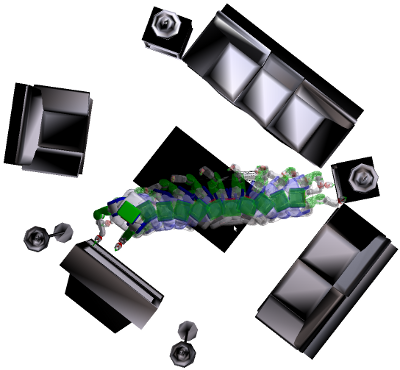
\includegraphics[width=0.48\linewidth]{figure/1.png}}
\subfloat[result path]{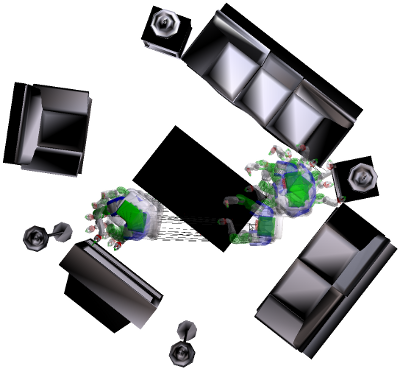
\includegraphics[width=0.48\linewidth]{figure/2.png}} \\
\subfloat[initial path]{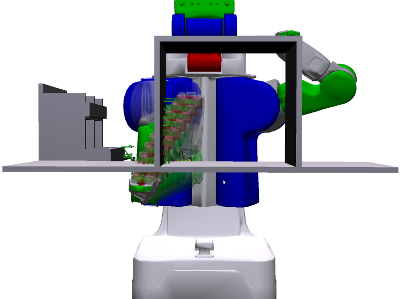
\includegraphics[width=0.48\linewidth]{figure/5.png}}
\subfloat[result path]{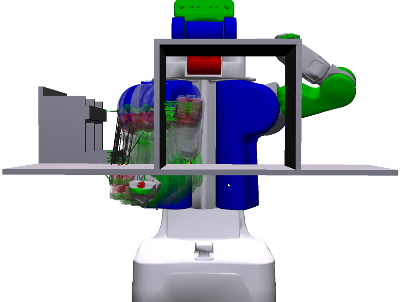
\includegraphics[width=0.48\linewidth]{figure/6.png}}
\caption{Failure cases when using the state-of-the-art trajectory optimization method~\cite{Schulman:2013:FLO} in motion planning. (a) shows the initial path for a whole-body planning, which passes through the medial axis of the desk obstacle. (b) is the trajectory optimization outcome, which is stuck in an infeasible condition. (c) shows the initial path for the arm planning and the collision cannot be resolved in the final trajectory shown in (d). }
\label{fig:failexamples}
\end{figure}



We propose a learning-based approach to predicting the quality of a trajectory as an initialization to trajectory optimization based motion planning. Quality is measured by whether the optimization converges to a collision free trajectory connecting start and goal. 
For the learning algorithm, we first design a set of trajectory features, which are relevant to a trajectory's effectiveness as an initialization. These features are both task-independent and scene-independent, and hence they are transferable among different planning tasks. We use three types of features: first, spatial signed distance (SSD) vectors for each robot link; second, the difference between SSD vectors for the same robot link in adjacent trajectory waypoints and for adjacent robot links in the same waypoint; and third, the spherical harmonics transform of SSD vectors. These features are able to encode the obstacle distribution locally around a robot trajectory and thus are essential for predicting a trajectory's behavior under a trajectory optimization algorithm. Next, we calculate the features for a set of randomly selected trajectories for different tasks in various benchmarks. To generate a labeled dataset, we run trajectory optimization for a large number of tasks and environments. Based on the dataset, we can learn a prediction function for trajectory effectiveness, which can be integrated with trajectory optimization algorithms to improve their solving performance and solution quality.

The rest of the paper is organized as follows. We survey related work on trajectory optimization and initial value selection for general optimization problems in Section~\ref{sec:related}. In Section~\ref{sec:probstatement}, we define the problem of predicting the quality of a trajectory as an initial guess. In Section~\ref{sec:predict}, we present the details about how to implement such prediction function using machine learning and a set of carefully selected features. Section~\ref{sec:experiment} describes the results of our method on various planning benchmarks.

\section{Related Work}
\label{sec:related}
Trajectory optimization is an established method in robotics to generate a high quality path from an initial trajectory that may be in-collision or dynamically infeasible; it works by solving an optimization problem on trajectory space. Many approaches use a spline-based or waypoint-based representation for the trajectory and use cost gradient information for minimization, including CHOMP~\cite{Ratliff:2009:CGO}, STOMP~\cite{Kalakrishnan:2011:STOMP} and TrajOpt~\cite{Schulman:2013:FLO}. There is extensive, closely-related work in optimal control. The optimal control literature focuses less on collisions and more on systems with complicated dynamical properties. Some of the most notable work includes DDP (Differential Dynamic Programming)~\cite{Jacobson:1970:DDP,Atkeson:1994:ULT}, Iterative LQR (iLQR)~\cite{Todorvo:2005:iLQG}, Approximate Inference Control~\cite{Toussaint:2009:RTO} and optimization-based control that involves contacts~\cite{Mordatch:2012:DCB,Tassa:2012:SSC,Erez:2012:TOD,Posa:2013:DTO}. 

One main challenge of trajectory optimization is that it is sensitive to the choice of initial trajectories and may get stuck in infeasible local optima. This is because the set of all collision-free configurations is highly non-convex, so the optimization is prone to getting stuck in local minima.

For general non-convex optimization problems, the dependence on initialization is also a well-known challenge. A simple and popular solution is using multiple random initializations to help the algorithms escape from bad local optima. 
Recent work~\cite{Cassioli:2012:MLG} uses machine learning to learn the relationship between the starting point of an optimization algorithm and the objective value of the final outcome and is closely related with our method. The main difference is that our approach is for trajectory optimization, where generating a feasible trajectory is more important than decreasing the absolute cost of the objective function. Moreover, trajectory optimization can exploit workspace or physics based heuristics for selecting good initial guesses, which are not available in general optimization problems.

Another closely related line of work is on trajectory prediction~\cite{Jetchev:2013:FMP}, where a high-dimensional feature vector is used to capture information about the proximity of a robot to the obstacles. After a sparse regularized feature selection process, machine learning algorithms are used to predict a good path in a new environment from the database of previous trajectories and environments. The predicted result may not be feasible and hence requires another trajectory optimization step to resolve all the constraint violations. This post-processing might fail as the predicted trajectory may be a bad initialization for trajectory optimization.

Prior work has also considered designing trajectory features for various applications. For example, Bentivegna et al.~\cite{Bentivegna:2006:LST} and Stolle et al.~\cite{Stolle:2007:TPT} represented a library of trajectories by their feature vectors in order to make control policy transfer more convenient. 
Berenson et al.~\cite{Berenson:2012:RPP} designed several criteria and features to evaluate 
whether a trajectory from a path library is likely to be reused in a new planning scene after suitable repair operations. Trajectory features can also be used to predict the class labels of moving objects based on their trajectories~\cite{Lee:2008:TTC}. Moreover, features have been designed to compress trajectory libraries~\cite{Arikan:2006:CMC}. However, all these features only capture properties of the trajectory itself. In contrast, the features proposed in our paper encode the interaction between the trajectory and the surrounding environment, which is critical for predicting how fast a trajectory will be pushed away from the obstacles by a trajectory optimization algorithm.




\section{Problem Definition}
\label{sec:probstatement}

Robotic motion planning problems can be formulated as non-convex optimization problems, i.e., minimize an objective subject to inequality and equality constraints:

\begin{equation*}
\begin{aligned}
& \underset{\x}{\text{minimize}}
& & f(\x) \\
& \text{subject to}
& & g_i(\x) \leq 0, \; i = 1, 2, \dots, n_{\text{ieq}} \\
&&& h_i(\x) = 0, \; i = 1, 2, \dots, n_{\text{eq}}
\end{aligned}
\end{equation*}
where $f$, $g_i$ and $h_i$ are scalar functions. For planning problems that involve only kinematics and represent the trajectory as a sequence of $T$ waypoints, the optimization variable $\x$ is of the form of $\x = \btheta_{1:T}$, where $\btheta_t \in \mathbb{R}^K$ denotes the configuration at the $t$-th waypoint for a system with $K$ degrees of freedom. For problems with dynamics, the optimization variable $\x$ may also include velocities $\dot{\btheta_t}$ and torques ${\bm \tau}_t$.


Collision avoidance is one of the most important inequality constraints in motion planning. But it is difficult to formulate in closed form and hence is challenging for optimization. Various approximations for collision avoidance constraints have been proposed, including distance fields~\cite{Khatib:1985:ROA, Ratliff:2009:CGO}, penetration depth~\cite{Cameron:1997:CMP}, and swept volume~\cite{Schulman:2013:FLO}. Besides collision avoidance, common inequality constraints include kinematic constraints (e.g., joint limits and static stability constraints), kinodynamic constraints (e.g., bounded velocity, acceleration or force/torque) or dynamic constraints (e.g., dynamic stability constraints). One example of equality constraints is the end-effector pose constraint where the robot must reach a target pose at the end of the trajectory.

The objective function $f(\x)$ is often chosen to be a quadratic form of $\x$. For example, a widely used objective function for kinematic planning is $f(\btheta_{1:T}) = \sum_{t=1}^T \|\btheta_{t+1} - \btheta_{t}\|^2$, which encourages minimum-length or smoothness in the final outcome~\cite{Schulman:2013:FLO,Ratliff:2009:CGO}.

Trajectory optimization is a challenging non-convex problem, and many approaches have been presented to solve it efficiently and effectively. Among them are sequential convex optimization~\cite{Schulman:2013:FLO}, covariant Hamiltonian optimization~\cite{Ratliff:2009:CGO}, and stochastic optimization~\cite{Kalakrishnan:2011:STOMP}. However, given an initial trajectory that contains collisions, these methods are not guaranteed to find a collision-free solution as the collision avoidance terms in the optimization are non-convex. Figure~\ref{fig:badgradient} shows some scenarios illustrating how trajectory optimization tends to get stuck in local optima that are not collision-free. 

\begin{figure}[t]
\centering
\subfloat[]{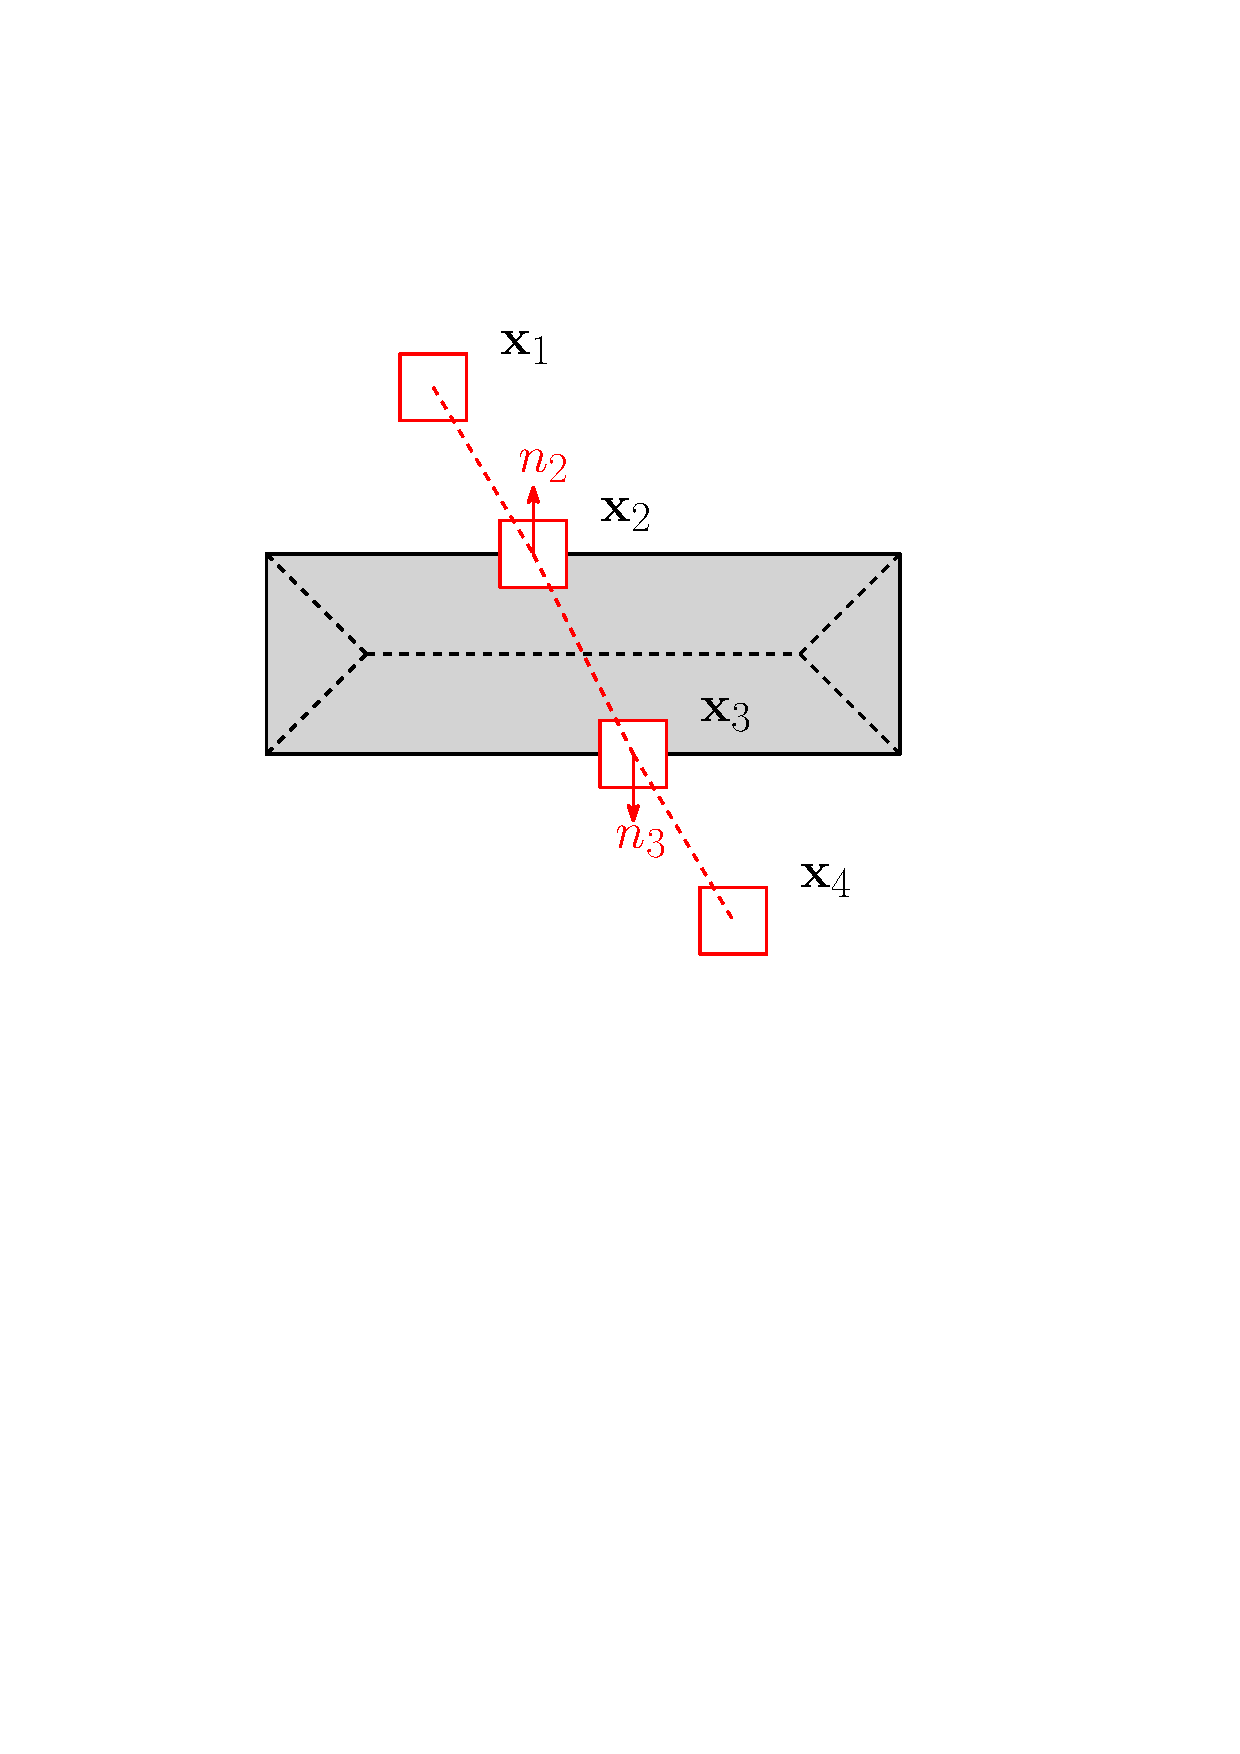
\includegraphics[width=0.42\linewidth]{figure/medial_axis.pdf}
}
\subfloat[]{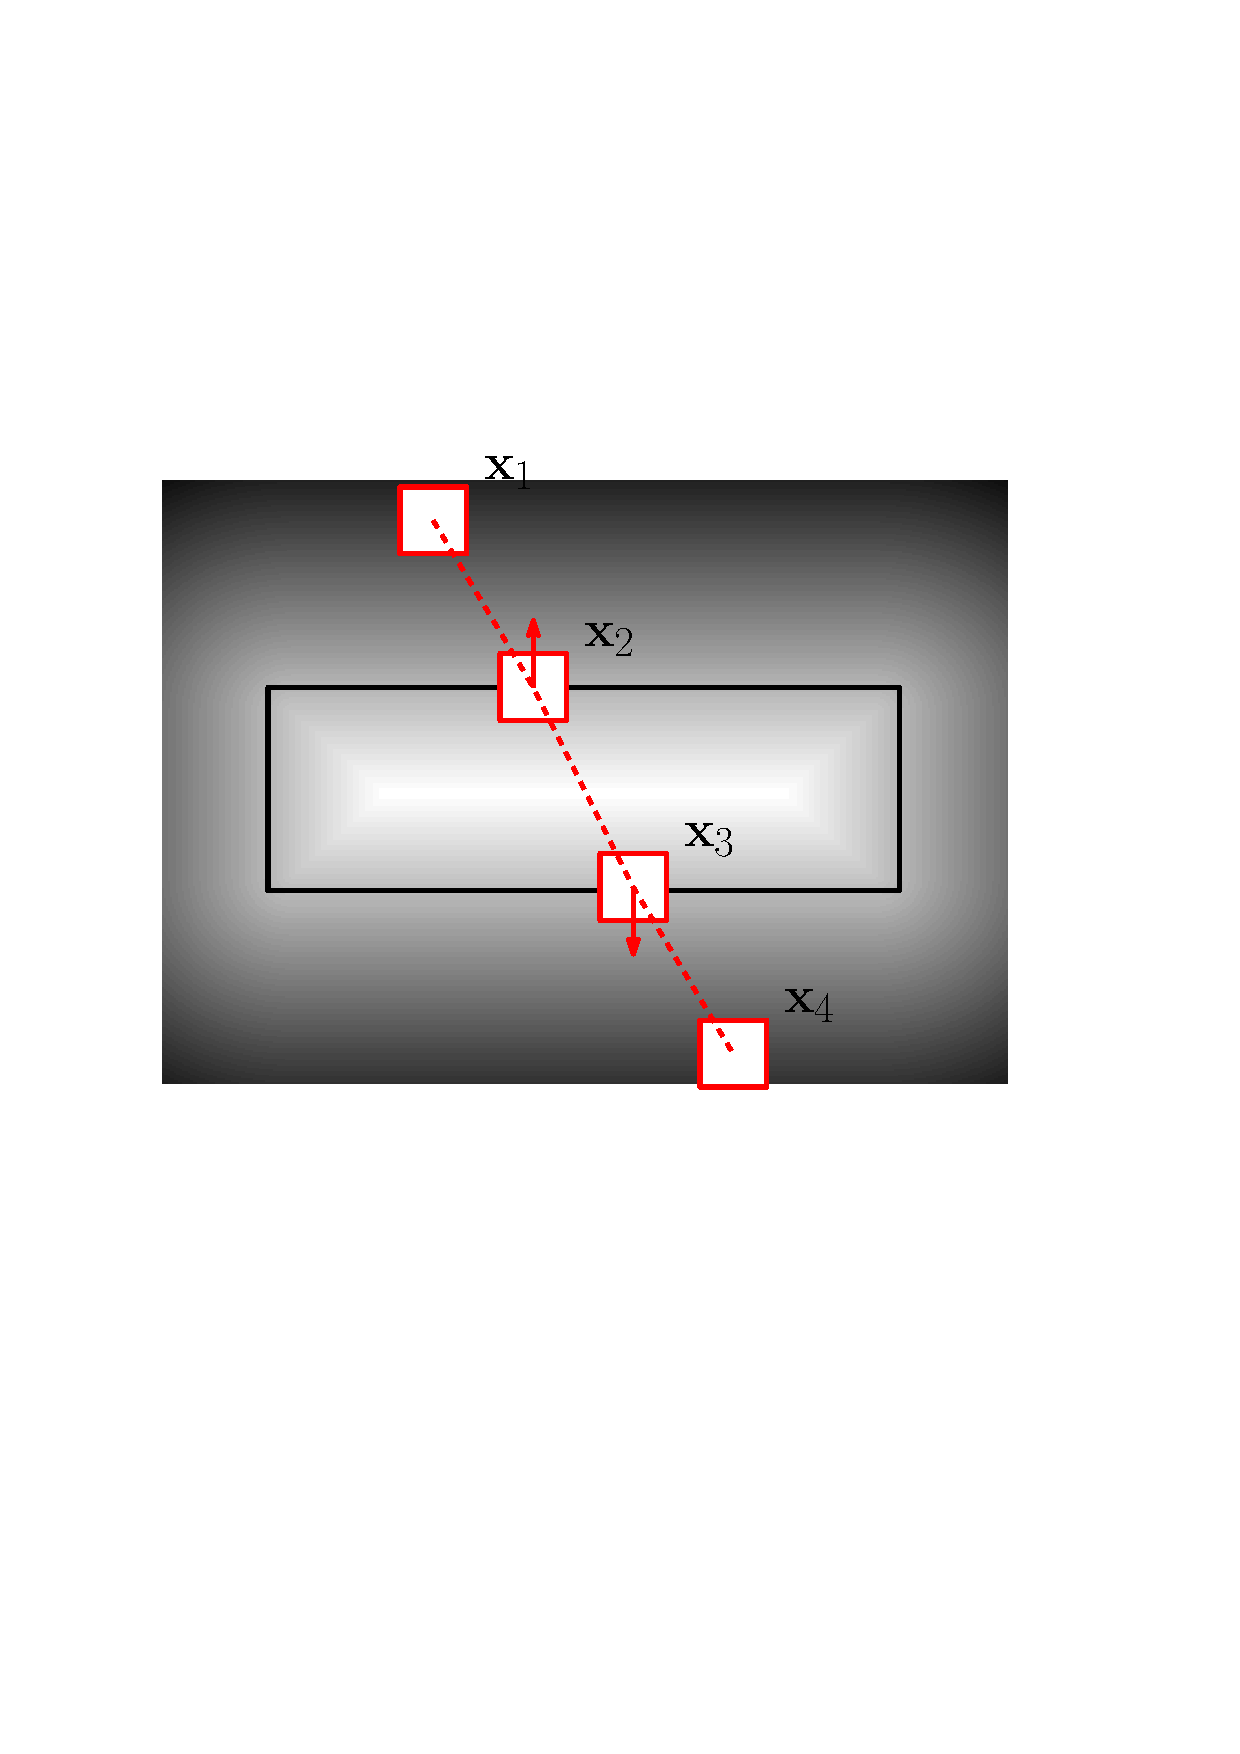
\includegraphics[width=0.55\linewidth]{figure/distance_field.pdf}} \\
\subfloat[]{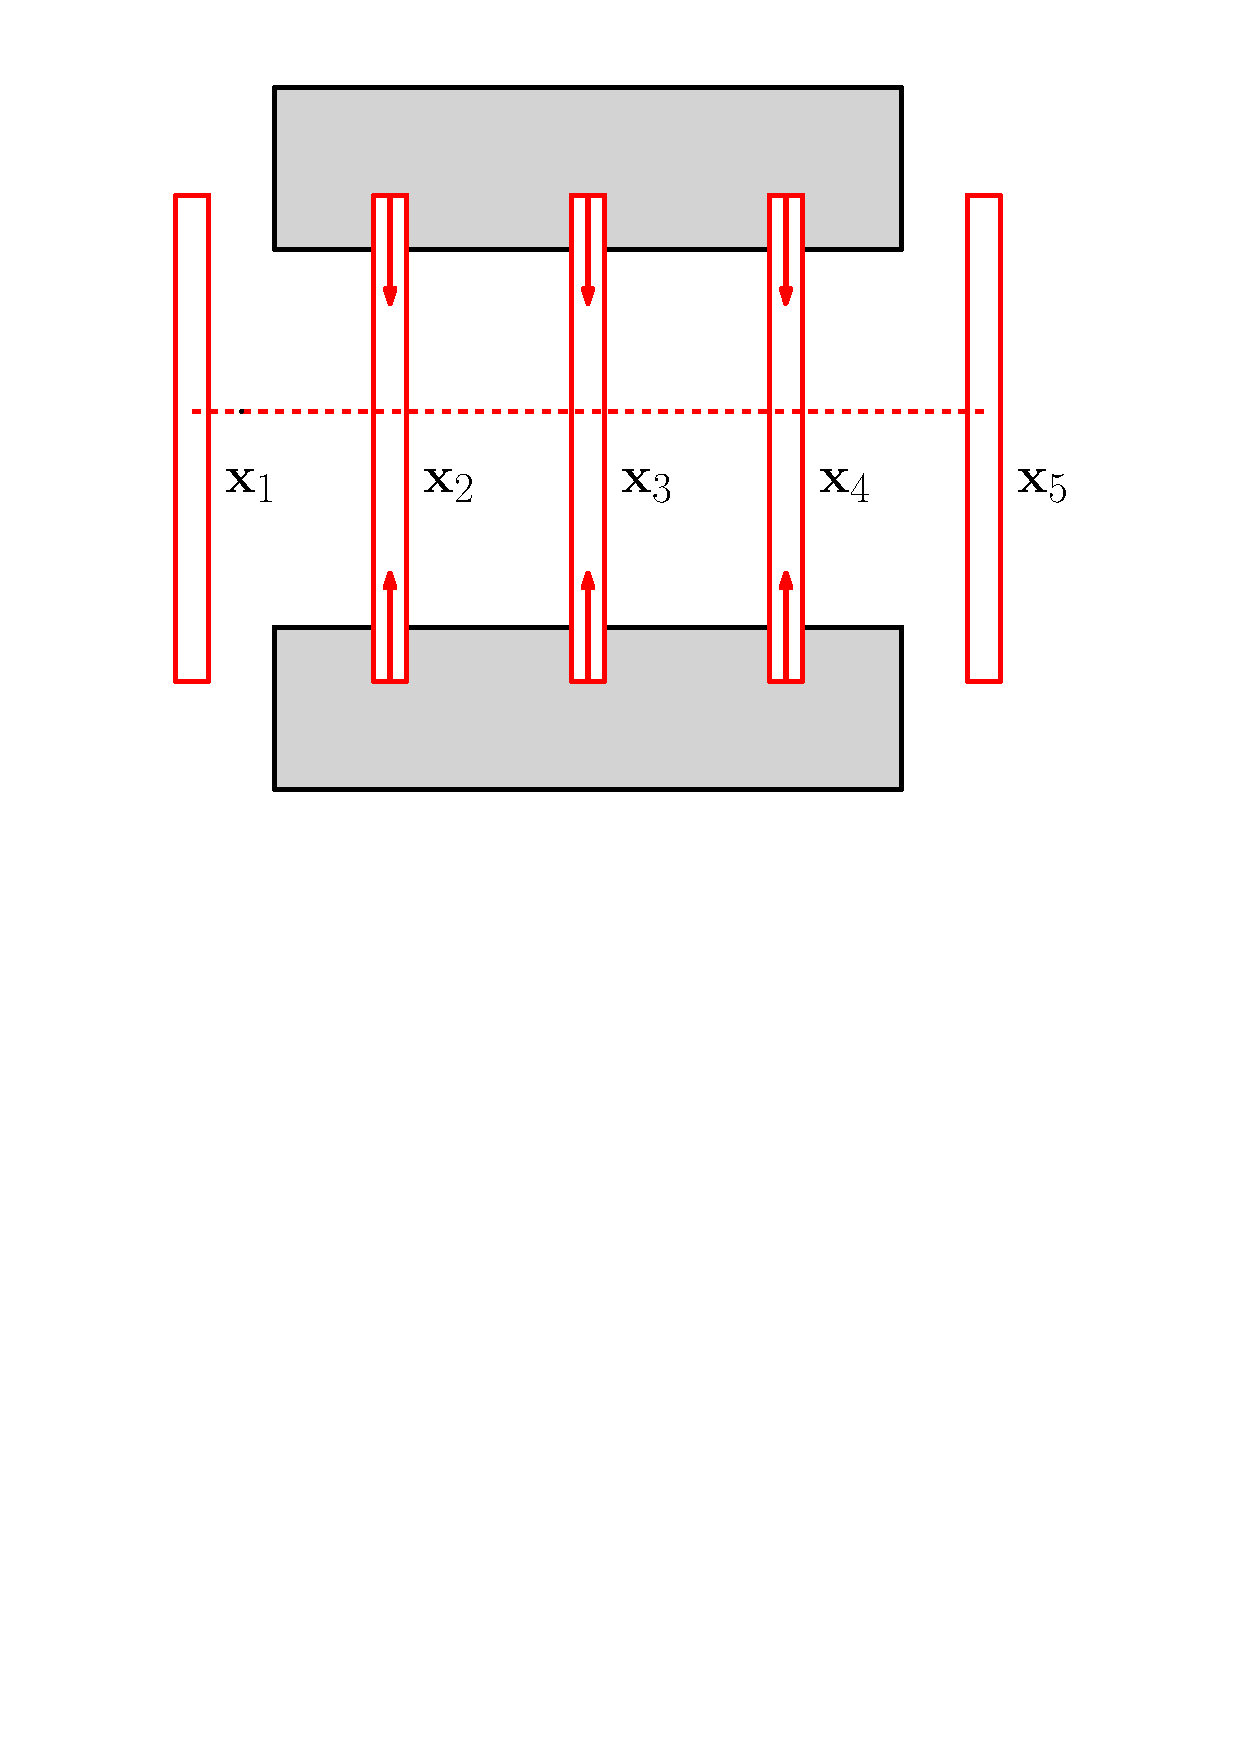
\includegraphics[width=0.48\linewidth]{figure/multiple_obstacle.pdf}}
\subfloat[]{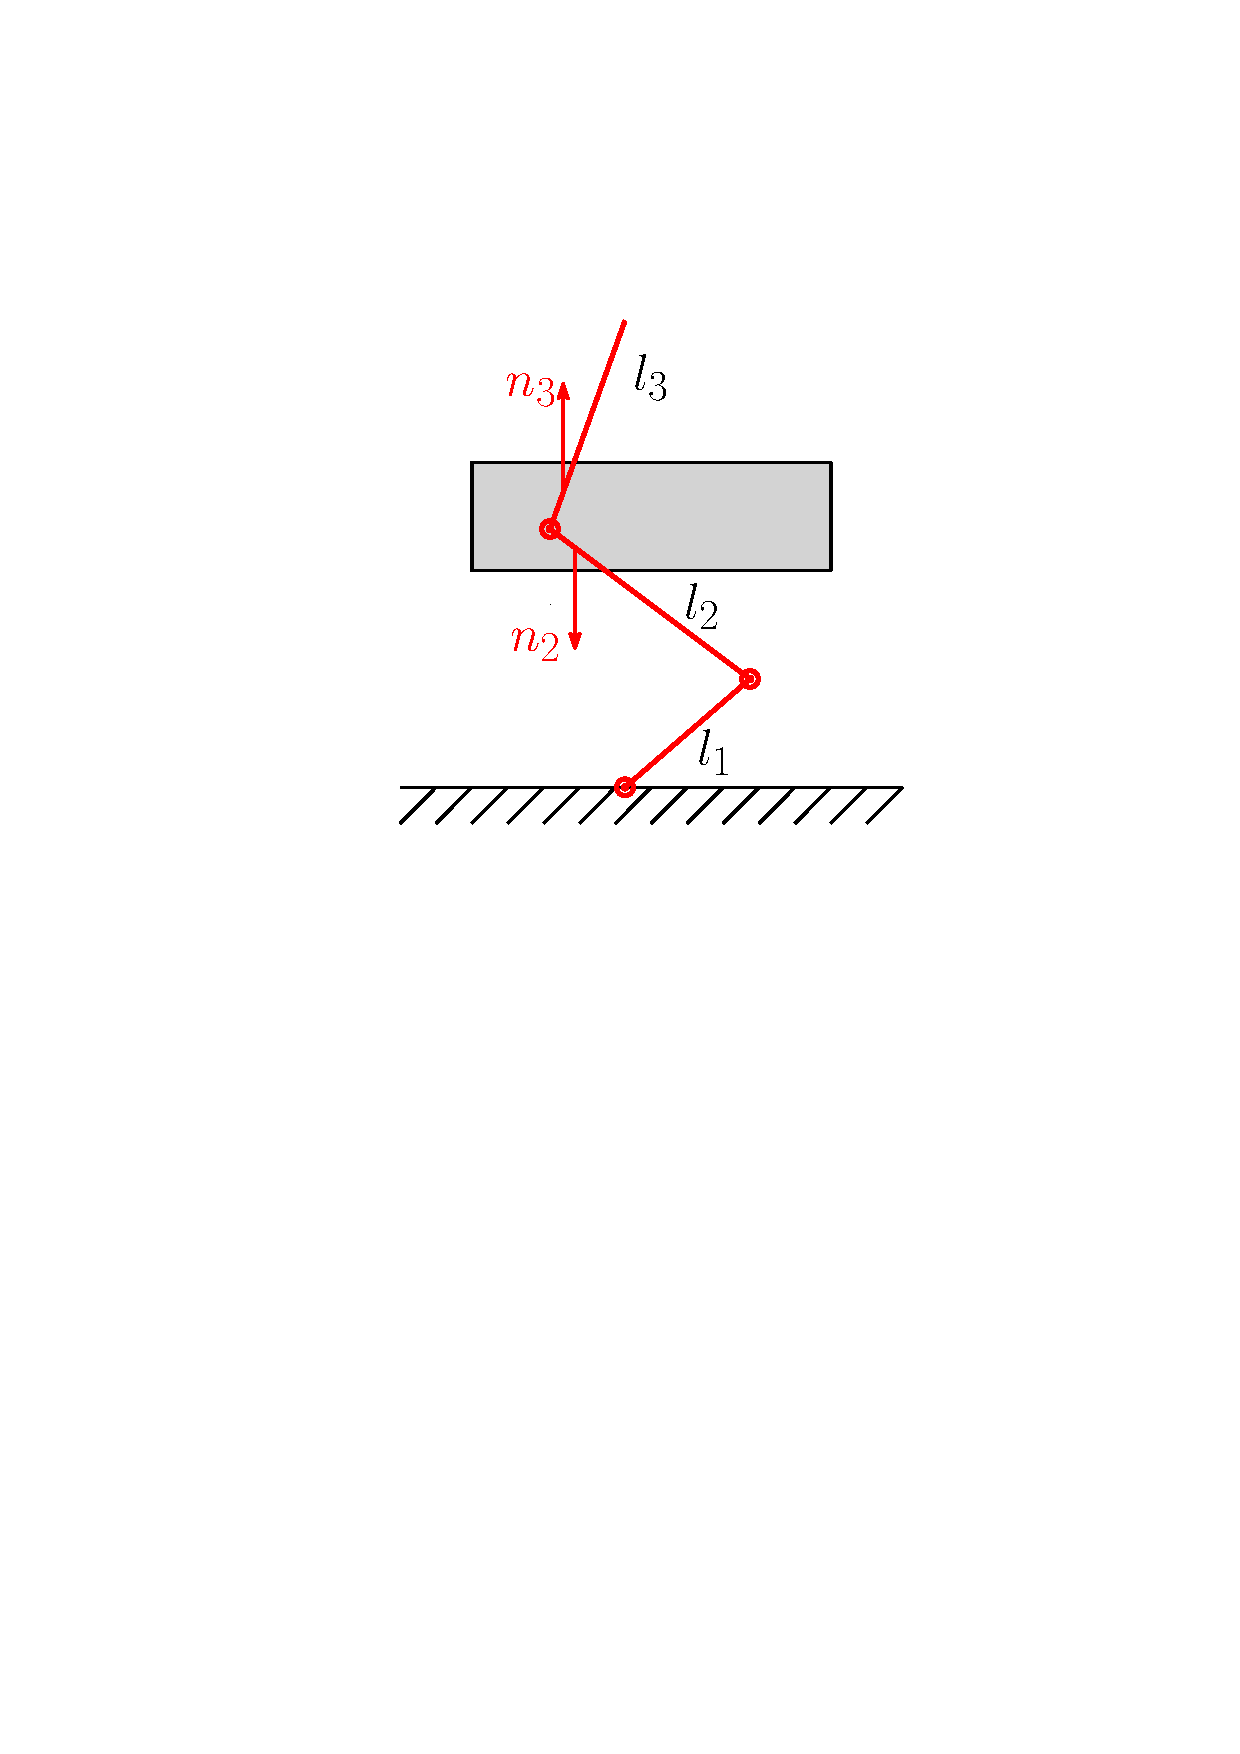
\includegraphics[width=0.48\linewidth]{figure/multiple_link.pdf}}
\caption{Illustration of typical reasons for trajectory optimization to get stuck in local optima that are not collision-free. (a) The gradient based on penetration depth may push waypoints in in-consistent directions. (b) The gradient based on distance fields has the same problem. (c) When a robot collides simultaneously with multiple obstacles, the robot may get stuck in an infeasible local optimum as different obstacles push the robot in different directions. (d) For a robot with multiple links, the gradient may result in in-consistent directions for different links. $\btheta_i$ in these figures denote different trajectory waypoints.}
\label{fig:badgradient}
\end{figure}

It is an on-going line of research to reshape the non-convex optimization formulations to improve their performance.  In this paper we consider the complimentary problem of: Given a trajectory optimization approach, how to predict which initializations will result in collision-free solutions and which ones will not. Such predictive capabilities would enable selecting a good initial trajectory for motion planning so that trajectory optimization is likely to converge to a collision-free local optimum. Such information can also be used to improve the performance of trajectory optimization being run in parallel for multiple initializations: For each solution sequence starting with a different initial guess, we can stop bad solution sequences early enough and focus computational budgets on solution sequences that potentially can converge to good outcomes.

\subsection{Outline of Proposed Approach}
We first design trajectory features that are potentially useful to distinguish good and bad initializations, which is based on the assumption that trajectories converging to feasible solutions share common properties. The features extracted from a trajectory $\btheta_{1:T}$ are denoted as a vector $\fsym = E(\btheta_{1:T})$, where $E(\cdot)$ is the extraction function. For each trajectory, we use a binary variable $y$ to denote whether the trajectory optimization succeeds ($y = 1$) or fails ($y = 0$).

Given a set of $N$ trajectories, we can build a training set $\{\fsym_i, y_i\}_{i=1}^N$. Based on the data set, we can learn a classifier $C(\fsym) = \{0, 1\}$, where $1$ means a feasible solution would be returned and the corresponding trajectory is potentially a good initial guess. The classifier $C(\cdot)$ is the predicator for a trajectory's effectiveness. 

\section{Predicting Initialization Effectiveness for Trajectory Optimization}
\label{sec:predict}

In this section, we discuss how to design trajectory features to distinguish good and bad initializations and how to use the extracted features to predict the effectiveness of a new trajectory.

Before extracting features from a trajectory, we first perform re-sampling on it so that the waypoints are uniformly distributed between two end-points. We perform this pre-processing based on what was pointed out by Ratliff et al.~\cite{Ratliff:2009:CGO}: the objective function should be invariant to the reparameterization of the trajectory so that the gradient will pull a trajectory out of obstacles instead of encouraging it to quickly jump through obstacles. Some recent work such as~\cite{Schulman:2013:FLO} handles the `jumping through problem' in a completely different way, but in practice, it is observed that a re-sampling pre-processing can still result in better convergence. Our re-sampling process excludes the difference of trajectories in parameterization and hence makes it easier to compare them. After re-sampling, each trajectory has $T$ waypoints. This also guarantees our feature extraction gives fixed-length vectors for different trajectories.

\subsection{Background: Signed Distances}
We design features to encode the obstacle distribution locally around a trajectory, as such information is closely related with a trajectory's effectiveness. Intuitively speaking, if a trajectory is deep inside the obstacles, it is less likely to be pushed out of them; whereas if it is mostly outside the obstacles, it should converge to a collision-free solution. To quantify the obstacle distribution surrounding a trajectory, we use signed distances and normals, which are used in previous trajectory optimization algorithms such as~\cite{Schulman:2013:FLO}. Formally, the signed distance is defined between two sets $\mathcal A$ and $\mathcal B$ in workspace as follows:
\begin{align}
\text{sd}(\mathcal A, \mathcal B) = \text{dist}(\mathcal A, \mathcal B) - \text{penetration}(\mathcal A, \mathcal B).
\end{align}
Here $\text{dist}(\mathcal A, \mathcal B)$ is the distance between $\mathcal A$ and $\mathcal B$, i.e., the length of the smallest relative translation $\mathbf T$ that puts these two non-overlapped sets in contact:
\begin{align}
\text{dist}(\mathcal A, \mathcal B) = \inf\{\|\mathbf T\| \mid (\mathbf T + \mathcal A) \cap \mathcal B \neq \emptyset\}.
\end{align}
And $\text{penetration}(\mathcal A, \mathcal B)$ is the (translational) penetration depth between $\mathcal A$ and $\mathcal B$, i.e., the minimum translation $\mathbf T$ that makes two overlapped sets out of contact:
\begin{align}
\text{penetration}(\mathcal A, \mathcal B) = \inf\{\|\mathbf T\| \mid (\mathbf T + \mathcal A) \cap \mathcal B = \emptyset\}.
\end{align}
The signed distance computation can be efficiently computed for convex objects using GJK algorithm~\cite{Gilbert:1988:GJK} and EPA algorithm~\cite{Bergen:2001:EPA}. Signed distance also provides a normal vector $\mathbf n = \frac{\mathbf T}{\|\mathbf T\|}$, i.e., the direction that two objects can be most efficiently pushed away from each other. Such a direction is important for a trajectory's effectiveness: As we showed in Figure~\ref{fig:badgradient}, a bad initialization tends to have adjacent waypoints with very different pushing away directions.


\subsection{Feature I: Spatial Signed Distance Vectors}
Based on the signed distances formulation, a natural choice for trajectory feature design is to collect the signed distances and normals between all pairs of robot links and environment obstacles, for each waypoint in the trajectory. More formally, given a robot with $n$ links $\mathcal A_i$ in an environment with $m$ obstacles $\mathcal B_j$, the feature vector would be $\fsd = \{\text{sd}_{i,j,t}, \mathbf n_{i,j,t}\}_{1\leq i \leq n, 1\leq j \leq m, 1\leq t \leq T}$, where $\text{sd}_{i,j,t} = \text{sd}(\mathcal A_i(t), \mathcal B_j)$ is the signed distance value between $\mathcal A_i$ and $\mathcal B_j$ at waypoint $\btheta_t$ and $\mathbf n_{i,j,t}$ is the corresponding normal. This feature vector has a dimension of $4\times m \times n \times T$ and indeed provides a complete description for the obstacle distribution around the trajectory, which is critical when predicting trajectory's effectiveness. However, the feature dimension will depend on $m$, the number of obstacles in the environment, which makes this feature not transferable between different environments. Moreover, in many real-world systems, there may be a large number of obstacles (e.g., the obstacles from sensor data are usually represented as thousands of boxes~\cite{Sucan:2010:CPT}). This will result in a long feature vector and brings challenges for both data storage and the following learning procedure. As a result, we need to summarize this feature in a more compact way but keep its rich information as much as possible. 

\begin{figure}[t]
\centering
\subfloat[]{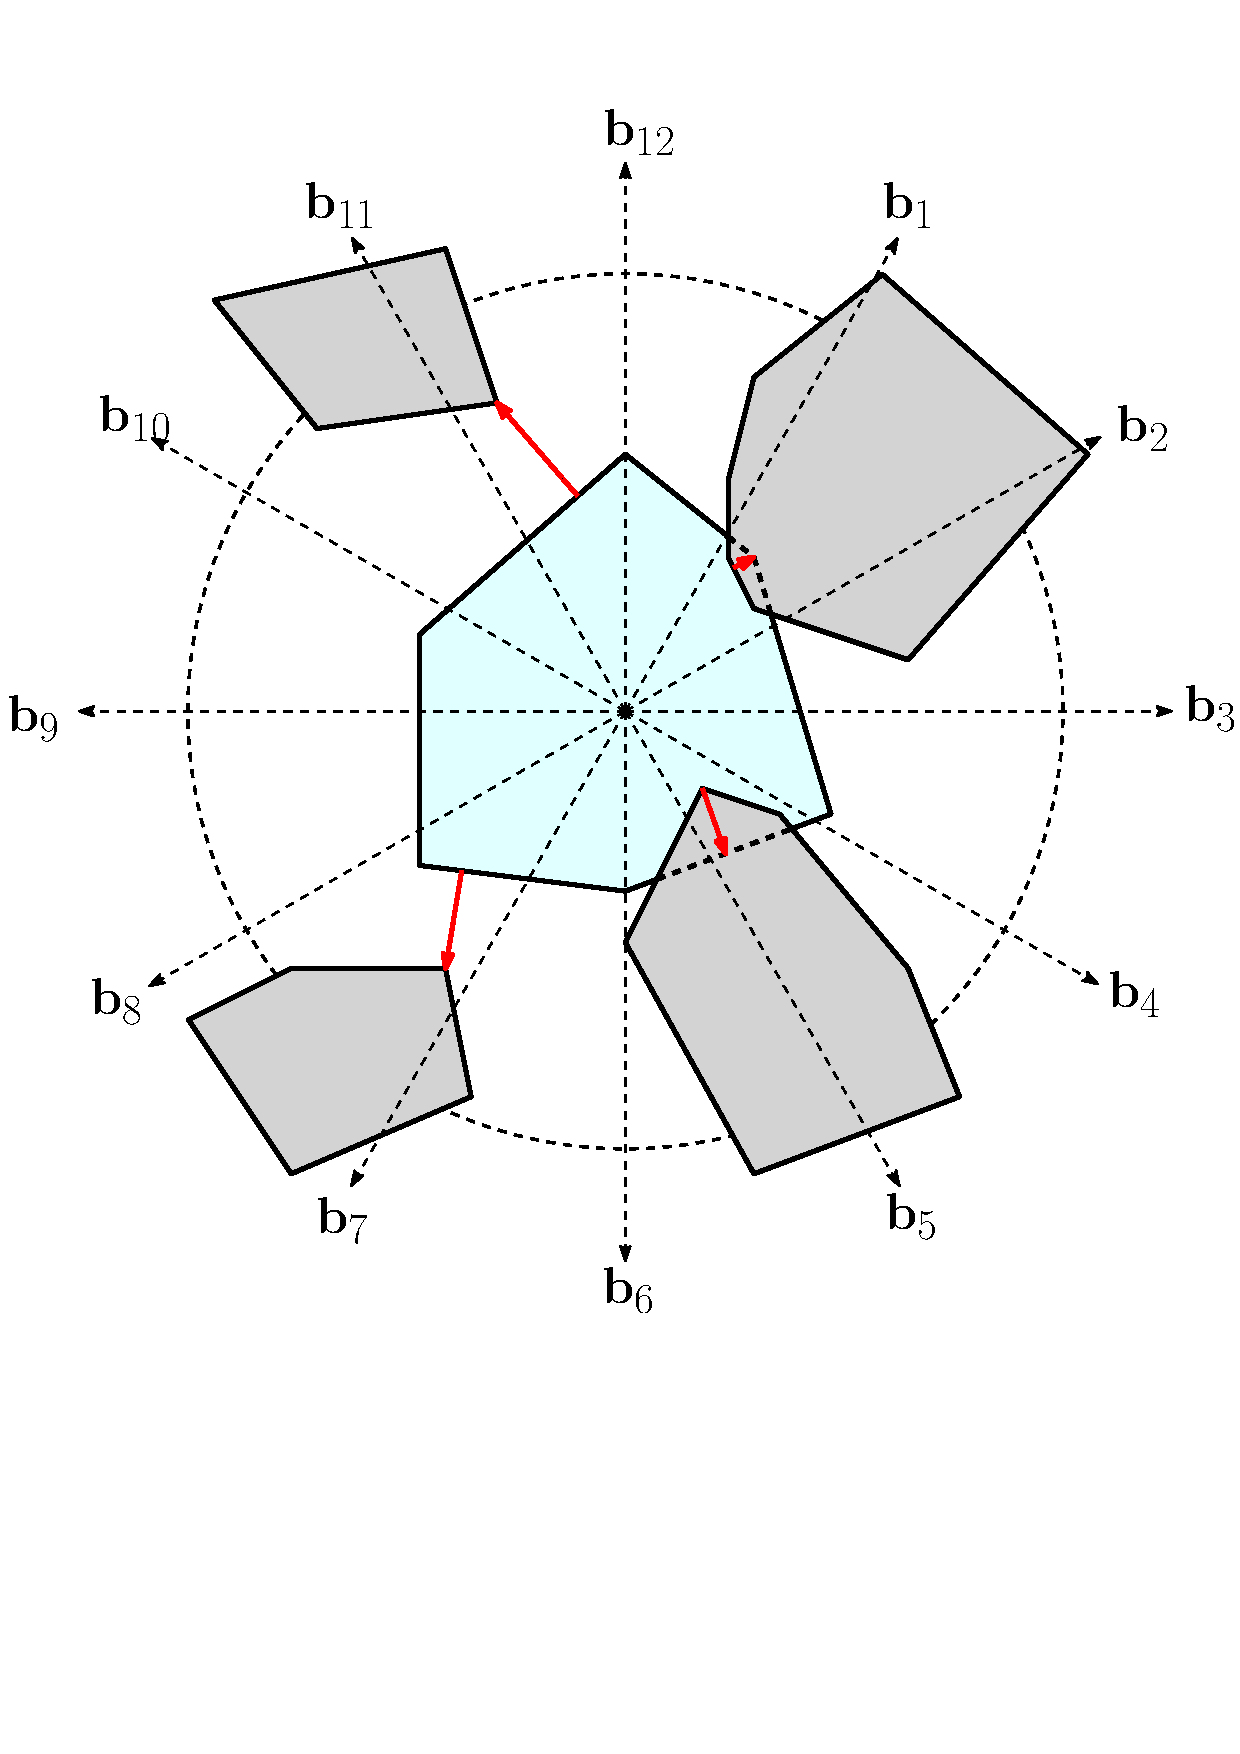
\includegraphics[width=0.52\linewidth]{figure/penetration_encode.pdf}}
\subfloat[]{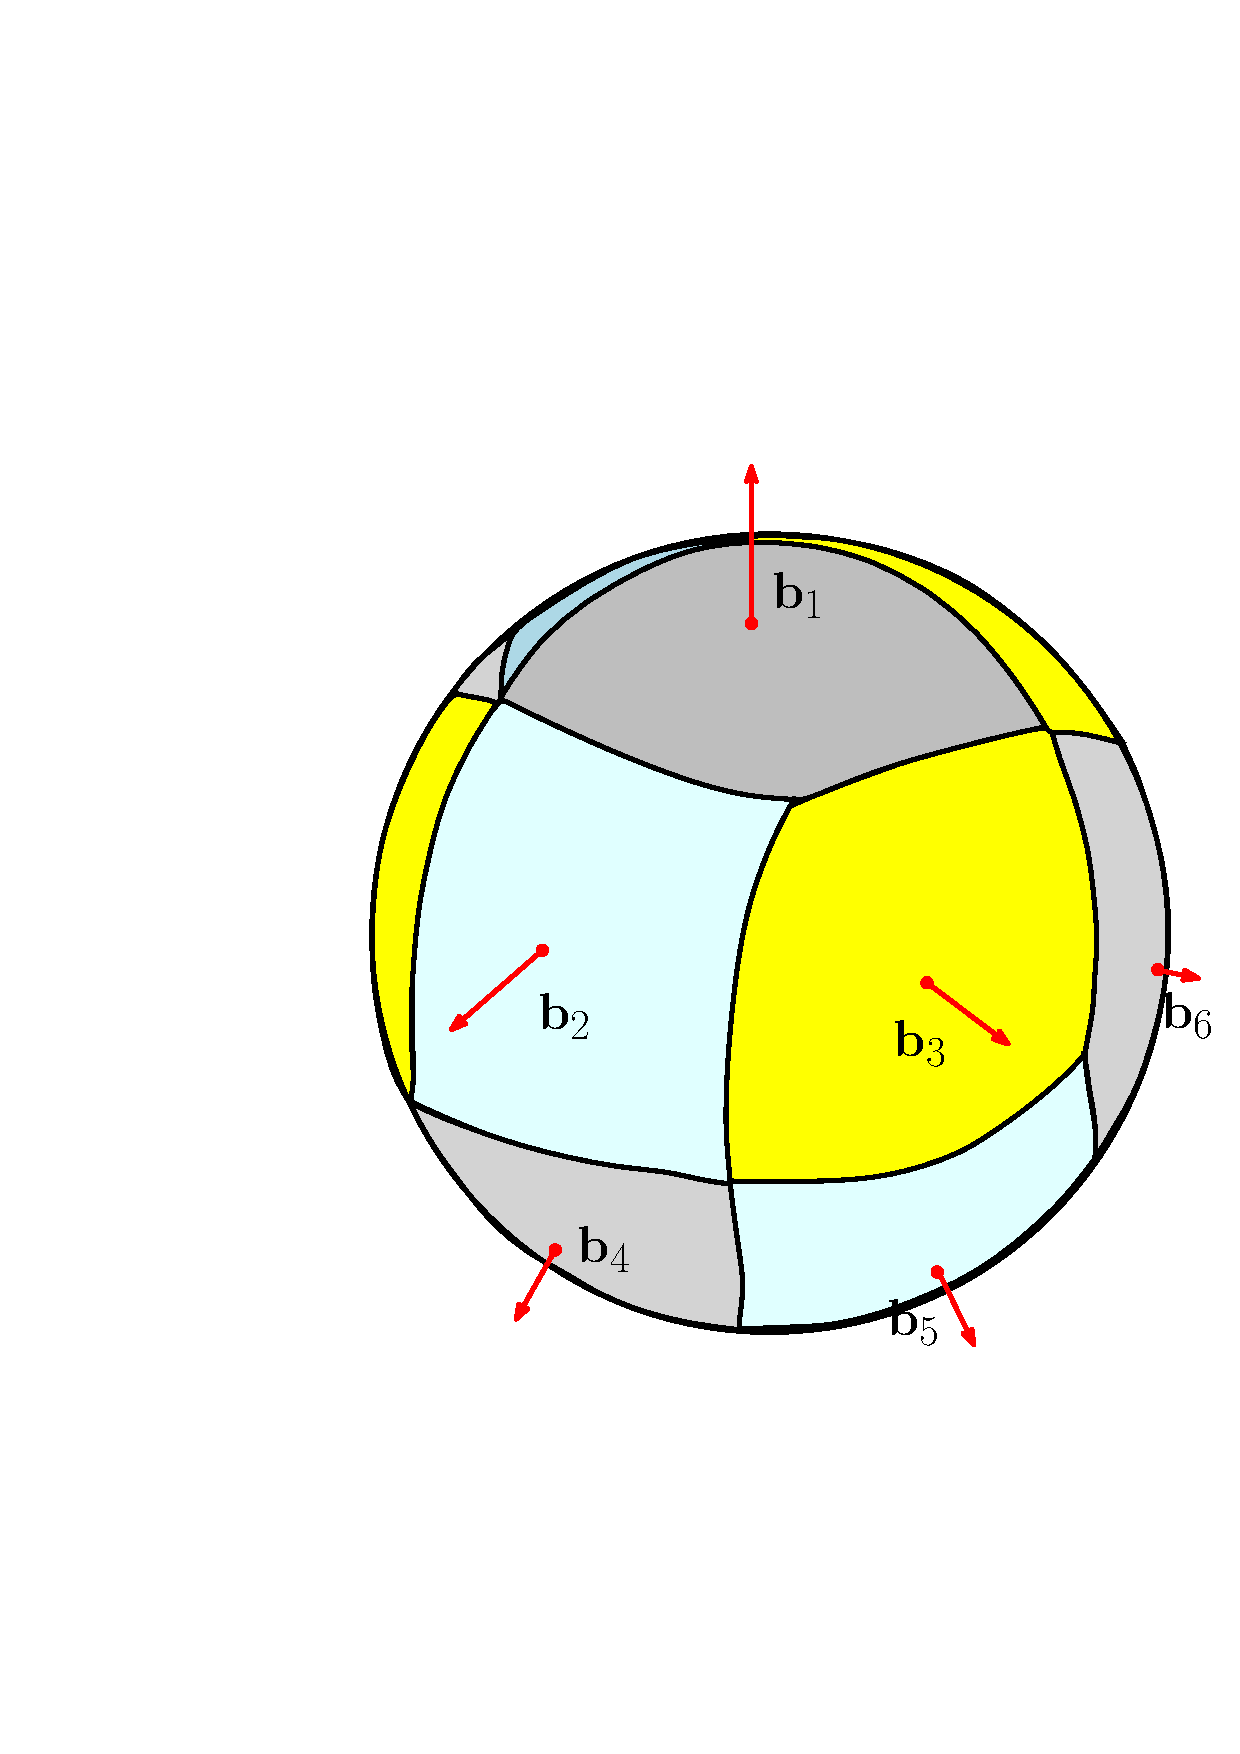
\includegraphics[width=0.47\linewidth]{figure/discrete_directions.pdf}}
\caption{Spatial signed distance vectors: (a) shows a 2D example about spatial signed distance vectors generation. The surrounding space around a robot link (the cyan color part) is uniformly divided by a spatial vector dictionary with $12$ prototype directions $\{\mathbf b_1, ..., \mathbf b_{12}\}$. The signed distance value $\text{sd}_j$ between the robot and the $j$-th obstacle (the grey parts) is then accumulated toward a prototype direction $\mathbf b_k$ which has the smallest angle with the corresponding signed distance normal $\mathbf n_j$, i.e., with the smallest $|\mathbf n_j \cdot \mathbf b_k|$. (b) In 3D case, we use the approach introduced in~\cite{Yershova:2010:GUI} to generate dictionary vectors that can make equisurface partition on a sphere surface. }
\label{fig:trajectoryfeaturePD}
\end{figure}



\begin{figure}[b]
\textbf{Input}: Signed distance values $\text{sd}_j$ and normals $\mathbf n_j$ between the robot link and the $m$ obstacles in the environment; The spatial vector dictionary of size $M$: $D = \{\mathbf b_1, ..., \mathbf b_M\}$\\
\textbf{Output}: Spatial signed distance vector $\fssd$
\begin{algorithmic}[1]
\State{Initialize $\fssd$ as a dimension-$M$ vector with default value $R$;}
\For{$j \leftarrow 1$ to $m$}
	\State{Find $\mathbf b_k$ in $D$ where $|\mathbf b_k \cdot \mathbf n_j|$ is the smallest;}
	\If{$\text{sd}_j < 0$ \text{and} $\fssd[k] < 0$}
		\State{$\fssd[k] \leftarrow \fssd[k] + \text{sd}_j$;}
	\Else
		\State{$\fssd[k] \leftarrow \min(\fssd[k], \text{sd}_j)$;}
	\EndIf
\EndFor
\end{algorithmic}
\label{algo:SSD}
\caption{SSD vector generation for one robot link at a trajectory waypoint}
\end{figure}

Our solution is to re-organize the signed distances and normals into a new form called the Spatial Signed Distance (SSD) Vectors. We illustrate the basic idea of SSD via a 2D example in Figure~\ref{fig:trajectoryfeaturePD}(a). We first partition the space around a robot link using a dictionary of direction vectors $D = \{\mathbf b_1, ..., \mathbf b_M\}$. These vectors are specially chosen so that when performing vector quantization for all the direction vectors in 2D, each dictionary vectors would have approximately the same number of directions closest to them. In other words, these dictionary vectors would divide the circle into bins with the same size. For 3D case, we use the approach introduced in~\cite{Yershova:2010:GUI} to generate the direction dictionary, which provides a uniform deterministic sequence of samples over $S^2$ (as shown in Figure~\ref{fig:trajectoryfeaturePD}(b)) based on a special multi-resolution grid structure. These dictionary directions will partition sphere surface into bins with the same size.

Given the signed distances and normals between the robot link and all the obstacles in the environment, we accumulate the signed distances along these discretized prototype directions in dictionary $D$ and the result is a $M$-dim vector $\fssd$. The $k$-th element of $\fssd$ is denoted as $\fssd[k]$, which measures how hard it is to push the link away from the obstacle along the direction $\mathbf b_k$. If $\fssd[k]$ is positive, then the link still has some distance from the obstacle and is safe; if $\fssd[k]$ is negative, then the link will go deeper inside the obstacle when being pushed in this direction and therefore should be pushed in the other directions. 


The algorithm to compute $\fssd$ based on signed distance information is shown in Figure~4. First, each element in $\fssd$ is initialized by a default value $R > 0$, which defines the size of the local neighborhood around the link. We use the robot link's bounding radius as $R$, which implies that a large object would have a larger local neighborhood. Next, suppose the $j$-th obstacle's signed distance to the robot link is $\text{sd}_j$ and the corresponding normal is $\mathbf n_j$. We first find the dictionary direction $\mathbf b_k$ which has the smallest angle with $\mathbf n_j$, i.e., quantizing $\mathbf n_j$ to the prototype direction $\mathbf b_k$ with the smallest $|\mathbf n_j \cdot \mathbf b_k|$. Then we merge $\text{sd}_j$ with the existing value in $\fssd[k]$. If both $\text{sd}_j$ and $\fssd[k]$ are negative, i.e., a new penetration is detected in a direction where the penetration was detected before, we add $\text{sd}_j$ onto $\fssd[k]$ to give a large penalty for such in-collision case. For other cases, we update $\fssd[k]$ by $\text{sd}_j$ if $\fssd[k]$'s current value is larger than $\text{sd}_j$. In other words, $\fssd[k]$ is with the signed distance value of the closest obstacle. If $\fssd[k]$ remains $R$ after the computation, this means that no penetration is detected within the given link's neighborhood along direction $\mathbf b_k$. In this way, we summarize the obstacle distribution information around a robot link into a length-$M$ SSD vector.

After computing the SSD vectors for all the links belonging to all trajectory waypoints, we combine them together into the SSD feature vector for the entire trajectory, which is of dimension $n\times M \times T$ and is also denoted as $\fssd$. For environments with many obstacles, $M \ll m$ and therefore $\fssd$ is more compact than $\fsd$.



\subsection{Feature II: Difference between Spatial Signed Distance Vectors}
Spatial signed distance feature provides a complete description about the obstacle distribution around the trajectory. However, as we mentioned in Section~\ref{sec:probstatement}, whether the signed distance normal is consistent between adjacent links or adjacent waypoints in an initial trajectory is also important for the convergence of a trajectory optimization algorithm. Therefore, we need to design features to measure the consistency between two spatial signed distance feature vectors. Given two vectors $\fssd^a$ and $\fssd^b$, we evaluate their consistency using their dot-product $\fssd^a \cdot \fssd^b$. This dot-product has a larger value when $\fssd^a[k]$ and $\fssd^b[k]$ are of the same sign for all $k$. And it has a smaller value when some $\fssd^a[k]$ and $\fssd^b[k]$ are of the opposite sign, i.e., the signed distance normals are not consistent in direction $\mathbf b_k$. We compute dot-product between the SSD vectors of the same link in adjacent waypoints and the adjacent links in the same waypoint. We collect all the results in a feature vector denoted as $\fcon$, i.e., the consistency feature.

\subsection{Feature III: Spherical Harmonics Spatial Feature}
Spatial signed distance feature is not rotation-invariant and this may be problematic.
For example, when both the environment and the trajectory are rotated by a given angle, the trajectory feature will be completely different, and therefore it would be difficult to transfer the learning result between different benchmarks. Another example is when the environment is symmetric (such as Figure~\ref{fig:benchmarks1}(c)), the lack of rotation-invariance in the feature may decrease the accuracy of the learning algorithm.

As shown in Figure~\ref{fig:trajectoryfeaturePD}(a), the spatial signed distance feature in fact is a function defined on a sphere around a robot link. To represent the feature in a rotation-invariant manner, we can utilize the mathematical concept of spherical harmonics and the same idea has been used in various applications, including computer vision~\cite{Frome:2004:ROR} and graphics~\cite{Kazhdan:2003:RIS}.


The theory of spherical harmonics says that any spherical function $s(\theta, \phi)$ can be expressed as a sum of complex spherical harmonic basis functions $Y_l^m$: 
\begin{equation}
s(\theta, \phi) = \sum_{l=1}^{\infty} \sum_{m=-l}^{l} a_l^m Y_l^m(\theta, \phi).
\end{equation}
According to the property of spherical harmonics transform, the amplitudes of the harmonic coefficients $\|a_l^m\|$ are invariant to any rotation in the azimuthal direction. Moreover, the amplitude of $s_l$, the $l$-th frequency component of the function $s$, is rotation-invariant under any rotations, where $s_l = \sum_{m=-l}^{l}a_l^m Y_l^m(\theta, \phi)$. The magnitude of $s_l$ can also be computed based on $a_l^m$: $\|s_l\|^2 = \sum_{m=-l}^l \|a_l^m\|^2$. We use $\|s_l\|$ as features in 3D benchmarks. In 2D case, we use $\|a_l^m\|$ as features as only azimuthal rotation is allowed in 2D and $\|a_l^m\|$ can provide richer information. As in previous work~\cite{Frome:2004:ROR,Kazhdan:2003:RIS}, we choose a bandwidth $b$ and store only $b$ lowest-frequency components in our spherical harmonics feature $\fsht$. More formally, the feature is defined as $\fsht = \{\|s_l\|\}$ in 3D and $\fsht = \{\|a_l^m\|\}$ in 2D, where $m = 0,...,l$ and $l = 0,...,b$.

\subsection{Feature IV: Convexity Features}
	Another category of features used measured the local convexity of the problem around the trajectory. Since trajopt takes local convex approximations around the trajectory at each iteration in the 'convexify' step, these features measure how close the approximations are. 

	We computed eigenvalues of Hessian matrices of cost and constraint functions at the trajectory. We computed the following features on the eigenvalues to measure their negativity i.e. the problem's local nonconvexity: $i.$ The minimum eigenvalue. $ii.$ The sum of negative eigenvalues. $iii.$ The maximum eigenvalue. $iv.$ The sum of all eigenvalues. We computed these 4 statistics for each cost and constraint function individually, and for all of them combined (e.g. the sum of all eigenvalues of all Hessian matrices), for a total of $4 \times [(number\ of\ cost\ functions) + (number\ of\ constraint\ functions) + 1)]$ convexity features. We collected the features in a feature vector denoted ${\bf z}_\textrm{conv}$.

\subsection{Trajectory Evaluation and Effectiveness Prediction}
To evaluate whether a trajectory is `good' or `bad' as the initial guess for the optimization, currently we use two simple criteria: a trajectory is justified as a `good' initialization if the optimization algorithm converges and the final outcome does not violate any constraints. 

Given a set of trajectories with their features and evaluation results, we can use any two-class classification algorithm to learn a classifier for the trajectory. As the dimension of our trajectory feature is high (larger than $200$), we choose the linear support vector machine~\cite{Fan:2008:LLL} as the classifier due to its simplicity and efficiency.

\section{Experiment and Evaluation}
\label{sec:experiment}
We experimentally evaluate the trajectory features that we designed and demonstrate the accuracy of our effectiveness prediction approach on various 2D and 3D benchmarks, as shown in Figure~\ref{fig:benchmarks1},~\ref{fig:benchmarks2} and~\ref{fig:benchmarks3}. The trajectory optimization algorithm we used in the experiment is TrajOpt~\cite{Schulman:2013:FLO}, which is one of the state-of-the-art trajectory optimization algorithms.

\subsection{Experiment Setting}
For each benchmark, we have a pre-defined set of task settings (the initial and goal configurations) as seed tasks. For PR2 benchmarks, we use the $198$ arm planning problems and $96$ full-body problems used in TrajOpt~\cite{Schulman:2013:FLO}. For dubins car benchmarks, we manually select a set of initial-goal configurations that should have feasible solutions. Next, we perturb the initial and goal configurations around these seed tasks to generate more random tasks. We filter out the invalid tasks where the initial or goal configurations are in-collision. We also filter out the trivial cases where the linear interpolation between initial and goal is collision-free. We did not randomly select tasks in the entire configuration space because this will incorrectly bias the classifier toward tasks that will hardly happen in real world robotics applications.

Given one planning task, we first generate a trajectory which is a simple linear interpolation between the initial and goal configurations. Next, we perform random perturbation of the trajectory waypoints and generate more random trajectories. For each of these trajectories, we run the trajectory optimization algorithm using it as the initial guess. When the optimization stops, we will obtain a sequence of trajectories. These intermediate trajectories can also be used as initializer and they would all have the same effectiveness label as the actual initial guess. As a result, if the optimization converges and the final outcome is feasible, we evaluate the given initial trajectory and all the intermediate trajectories as `good' initializer. Otherwise we evaluate all of them as `bad'. Finally, we extract the features for all these labeled trajectories and add them into the dataset. In this way, we can generate more than $10,000$ trajectories for each planning benchmark. For each benchmark, we use half the data to train a classifier and the rest for testing experiments below. When splitting the training and test sets, we make sure that the trajectories corresponding to the same task are assigned into the same set. In this way, we guarantee that the test set is independent with the training set.
In Figure~\ref{fig:features}, we visualize the features of two trajectories from different benchmarks.

\subsection{Effectiveness Prediction on Same Benchmarks}
We first show the accuracy when using a classifier learned on one benchmark to predict the effectiveness of trajectories in the same benchmark but for different tasks. The results are shown in Table~\ref{tab:result}, where we compare the baseline accuracy and the accuracy when different combinations of features are used to train a classifier. From the results, we can see that the learned classifiers can provide accuracy significantly higher than the baseline (i.e., simply predicting the majority label in the training set), though different combinations of features may behave the best on different benchmarks.



\subsection{Effectiveness Prediction on Different Benchmarks}
A more challenging test is to check whether a classifier learned on one benchmark is able to correctly predict the effectiveness for trajectories from another benchmarks. For this test, we only obtain partial success: We indeed observe several successful transfers among different benchmarks as shown in Table~\ref{tab:result2}. However, for most cases, the prediction accuracy is low when the classifier is applying to a different benchmark.

There are several reasons for the transfer performance of the current prediction algorithm. First, our current feature design only considers the spatial information locally around the trajectory and does not take into account the global description about the environment, which has been proved to be helpful in movement transferring between different environments~\cite{Jetchev:2013:FMP}. For example, the classifier learned on squared-dubin in Figure~\ref{fig:benchmarks1}(c) can be successfully transferred to jagged-dubin in Figure~\ref{fig:benchmarks1}(a) because the environments are similar. The transfer to gap-dubin in Figure~\ref{fig:benchmarks1}(b) is difficult because the existence of the narrow gap. Second, for a high-DOF robot, the robot may use different part of DOFs in different scenarios and therefore different benchmarks may have different trajectory distributions. We need more trajectory data from different scenarios and different tasks in order to completely cover the trajectory space. Finally, the rotation-invariance of features is also important for transfer. From the successful case shown in Table~\ref{tab:result2}, we observe that the feature combination $\fcon+\fsht$ behaves the best in transferring, and both of them are rotation-invariant features. 

\begin{figure*}[t]
\centering
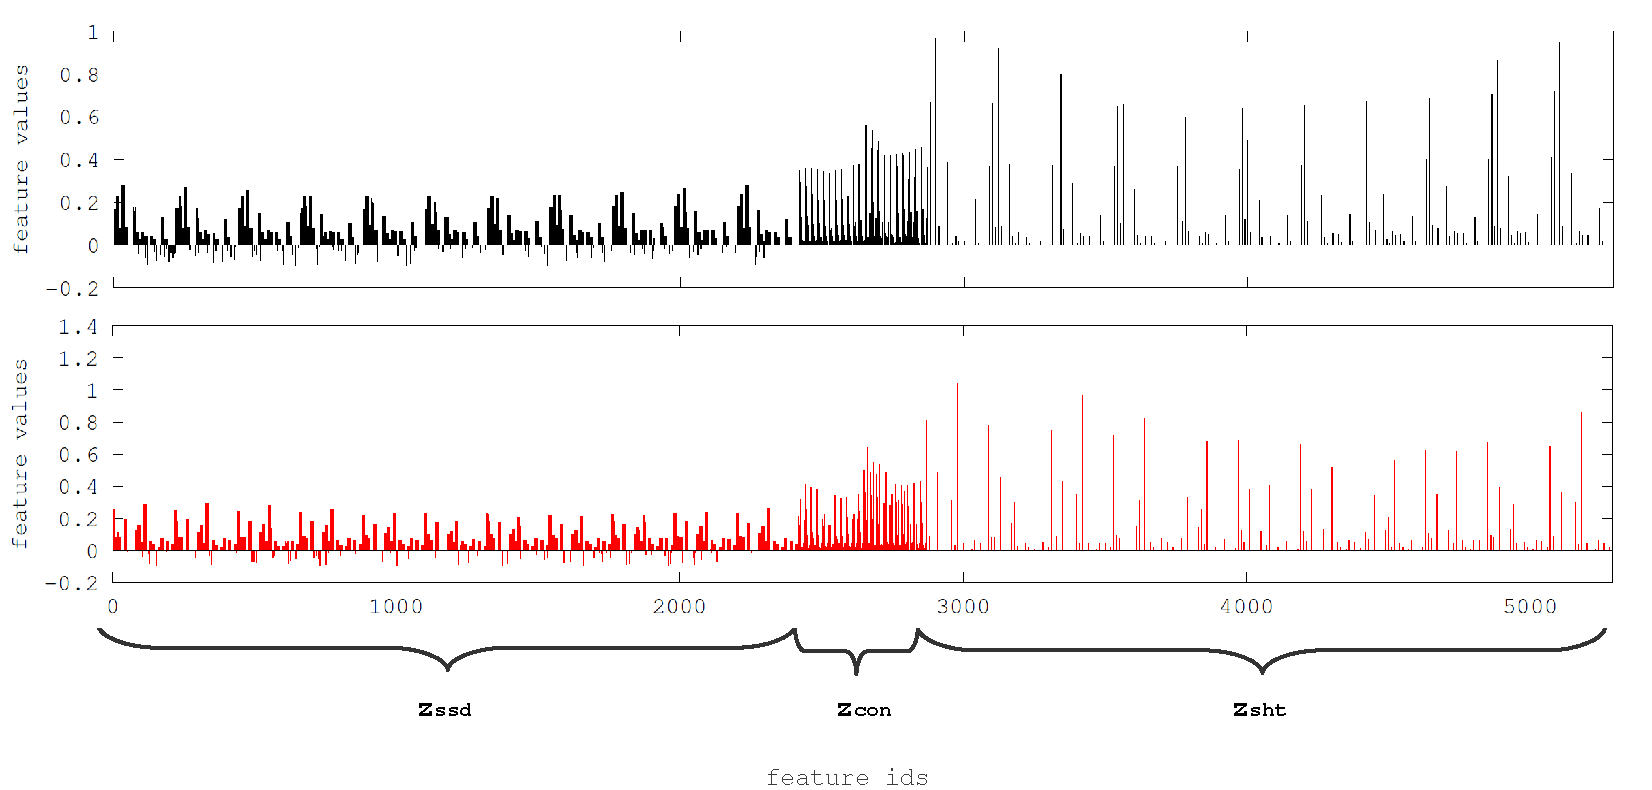
\includegraphics[width=\linewidth]{figure/features.pdf}
\caption{Features for two different trajectories in the bookshelf benchmark. Rough periods appears for all the three sub-features $\fssd$, $\fcon$ and $\fsht$, because these features are computed for each trajectory waypoint.}
\label{fig:features}
\end{figure*}

\begin{table*}[tbp]
\rowcolors{1}{gray!25}{}
\centering
\begin{tabular}{|c|r|r|r|r|r|r|r|r|}
\hline 
 & baseline & $\fssd+\fcon+\fsht$ & $\fssd+\fcon$ & $\fcon+\fsht$ & $\fssd+\fsht$ & $\fssd$ & $\fcon$ & $\fsht$ \\ \hline \hline
jagged-dubin & 59.2 & 82.6	& 82.2 & 74.7 & 82.3 & 82.2 & 70.1 & 63.15 \\ \hline
gap-dubin & 56.4 & 88.6 & 87.9 & 77.3 & 86.2 & 87.1 & 76.2 & 76.0 \\ \hline
squared-dubin & 56.8 & 89.3 & 	87.1 & 	77.5 &	88.2 &	85.0 &	 61.7	& 61.5 \\ \hline \hline

bookshelf & 63.0 & 77.7 & 	77.5 &	73.9 &	77.5 &	76.3 &	68.7 & 70.0 \\ \hline
skew-bookshelf & 62.1 & 80.4 &	74.3 & 	77.9 & 	76.2 &	72.3 &	63.7 &	65.0 \\ \hline
countertop & 69 & 70.1	& 72.8 & 	74.5	 & 69.6 & 	73.9 &	77.7 &	63.6 \\ \hline
industrial & 67.2 & 78.5 &	78.2 &	78.4 &	78.2 &	76.9 &	80.2 & 	73.7 \\ \hline
industrial2 & 50.3 & 61.1 & 	62.1	 & 64.1 &	61.2 & 	62.3 & 	64.5 &	58.2 \\ \hline \hline

livingroom & 61.0 & 85.5	& 88.4 &	 83.6 &	84.7 &	87.4 & 	82.8 &	81.6 \\ \hline
livingroom2 & 53.7 & 80.3 &	 80.5	& 76.7 &	 78.6 &	77.9 & 	71.5 & 	66.6 \\ \hline
kitchen & 59.0 & 65 & 	64.2 & 	60.4 &	66.9 & 	66.2 & 	60.3 & 	73.6 \\ \hline
kitchen2 & 54.0 & 64.6 &	65.3 & 	61.6 & 	65.0 & 	65.0 & 	61.0 &	61.5 \\ \hline
hotel & 98 & 98.1 &	98.1 & 	98.2 &	98.1 &	98.1 &	97	& 98.1 \\ \hline
\end{tabular}
\caption{The effectiveness prediction accuracy (in \%): We compare the prediction accuracy of the baseline (i.e., the percentage of majority trajectory label) with the prediction results when using all the features we designed $\fssd+\fcon+\fsht$ and all the other combinations of features.}
\label{tab:result}
\end{table*}

\begin{table*}[tbp]
\rowcolors{1}{gray!25}{}
\centering
\begin{tabular}{|c|r|r|r|r|r|r|r|r|}
\hline 
 & baseline & $\fssd+\fcon+\fsht$ & $\fssd+\fcon$ & $\fcon+\fsht$ & $\fssd+\fsht$ & $\fssd$ & $\fcon$ & $\fsht$ \\ \hline \hline
jagged-dubin to squared-dubin &  56.8 & 49.7 & 49.0 &	74.4 & 	56.9 & 	60.3	 & 67.9	& 55.5
 \\ \hline
squared-dubin to jagged-dubin & 59.2 & 56.9 &	56.8 &	71.1 & 	56.9 &	56.9 &	61.2 &	63.8 \\ \hline
bookshelf to skew-bookshelf & 62.1 & 57.1 &	59.4 &	82.1 & 	53.2 &	57.3 &	60.3 &	67.4 \\ \hline
\end{tabular}
\caption{The effectiveness prediction accuracy (in \%) when applying the classifier learned on one benchmark onto trajectories from other benchmarks. The baseline is the percentage of majority trajectory label of the benchmark where the classifier is transferred to.}
\label{tab:result2}
\end{table*}



\begin{figure*}[t]
\centering
\subfloat[jagged-dubin]{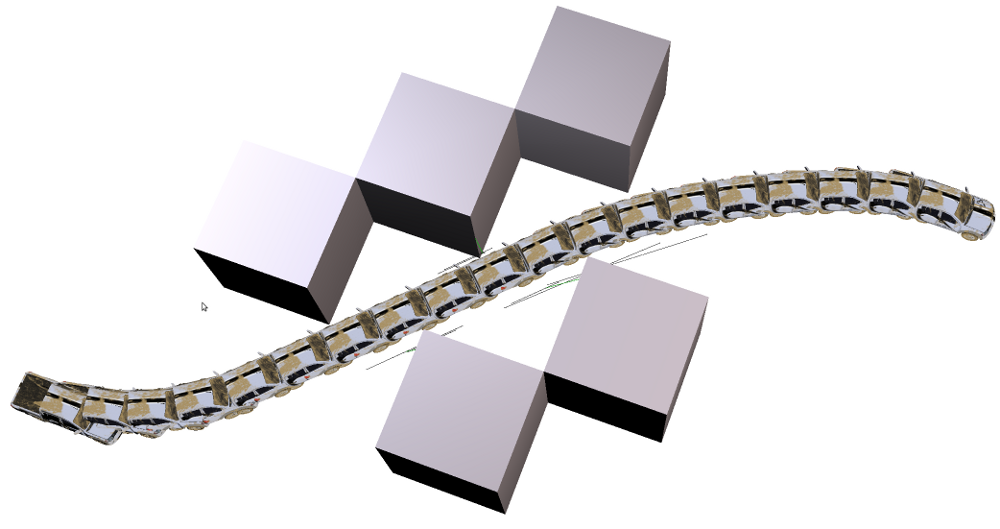
\includegraphics[width=0.33\linewidth]{figure/benchmark/jagged_dubins.png}}
\subfloat[gap-dubin]{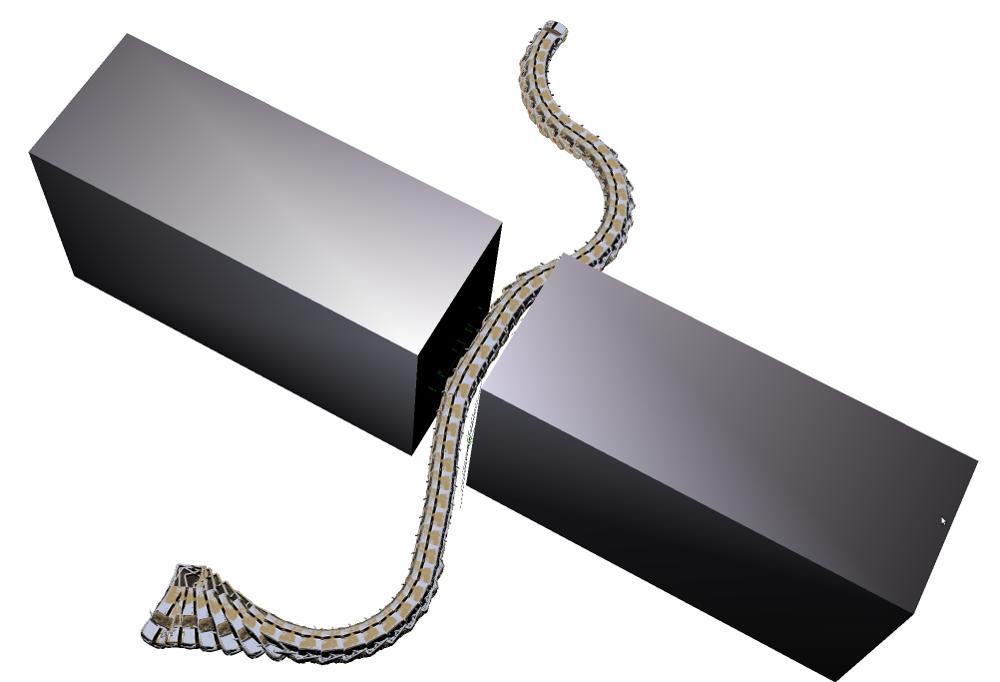
\includegraphics[width=0.26\linewidth]{figure/benchmark/cargap_dubins.png}}
\subfloat[squared-dubin]{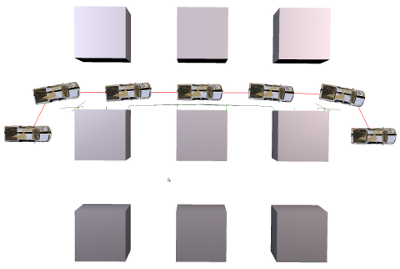
\includegraphics[width=0.27\linewidth]{figure/benchmark/squared_dubins.png}}
\caption{The dubins car environment for 2D experiments}
\label{fig:benchmarks1}
\end{figure*}

\begin{figure*}[t]
\centering
\subfloat[bookshelf]{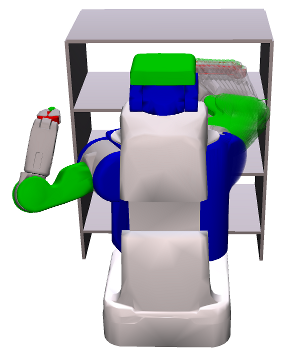
\includegraphics[width=0.15\linewidth]{figure/benchmark/bookshelves.png}}
\subfloat[skew-bookshelf]{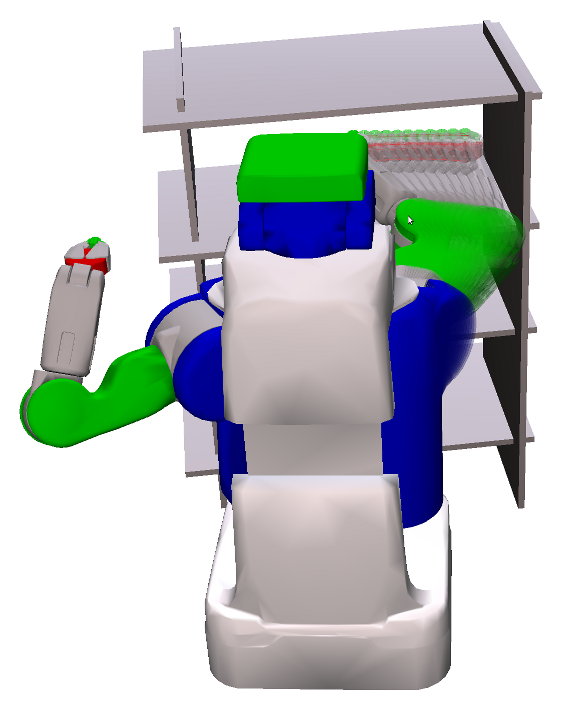
\includegraphics[width=0.15\linewidth]{figure/benchmark/bookshelves_rotate.png}}
\subfloat[countertop]{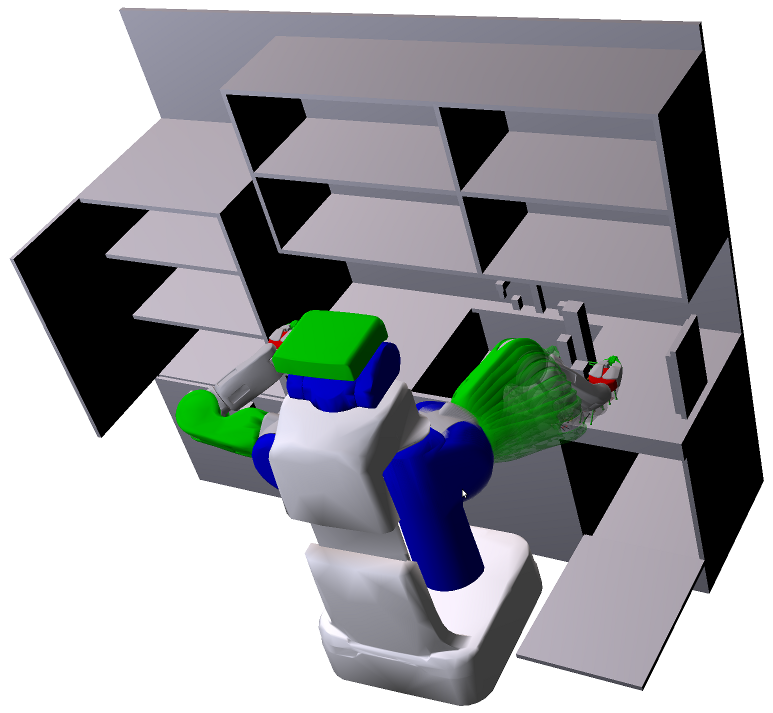
\includegraphics[width=0.20\linewidth]{figure/benchmark/countertop.png}}
\subfloat[industrial]{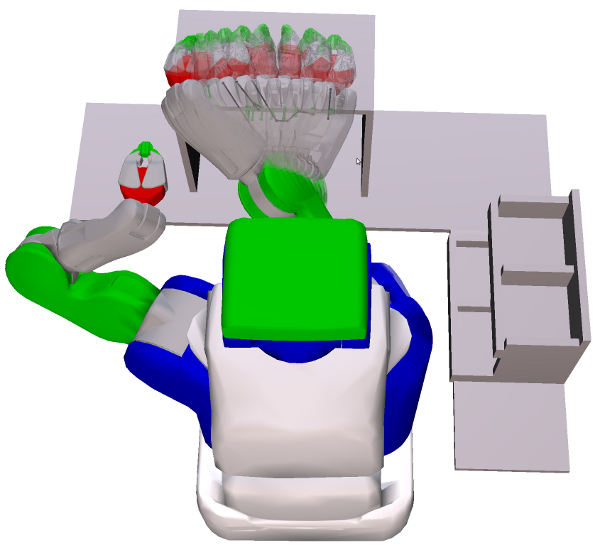
\includegraphics[width=0.20\linewidth]{figure/benchmark/industrial.png}}
\subfloat[industrial2]{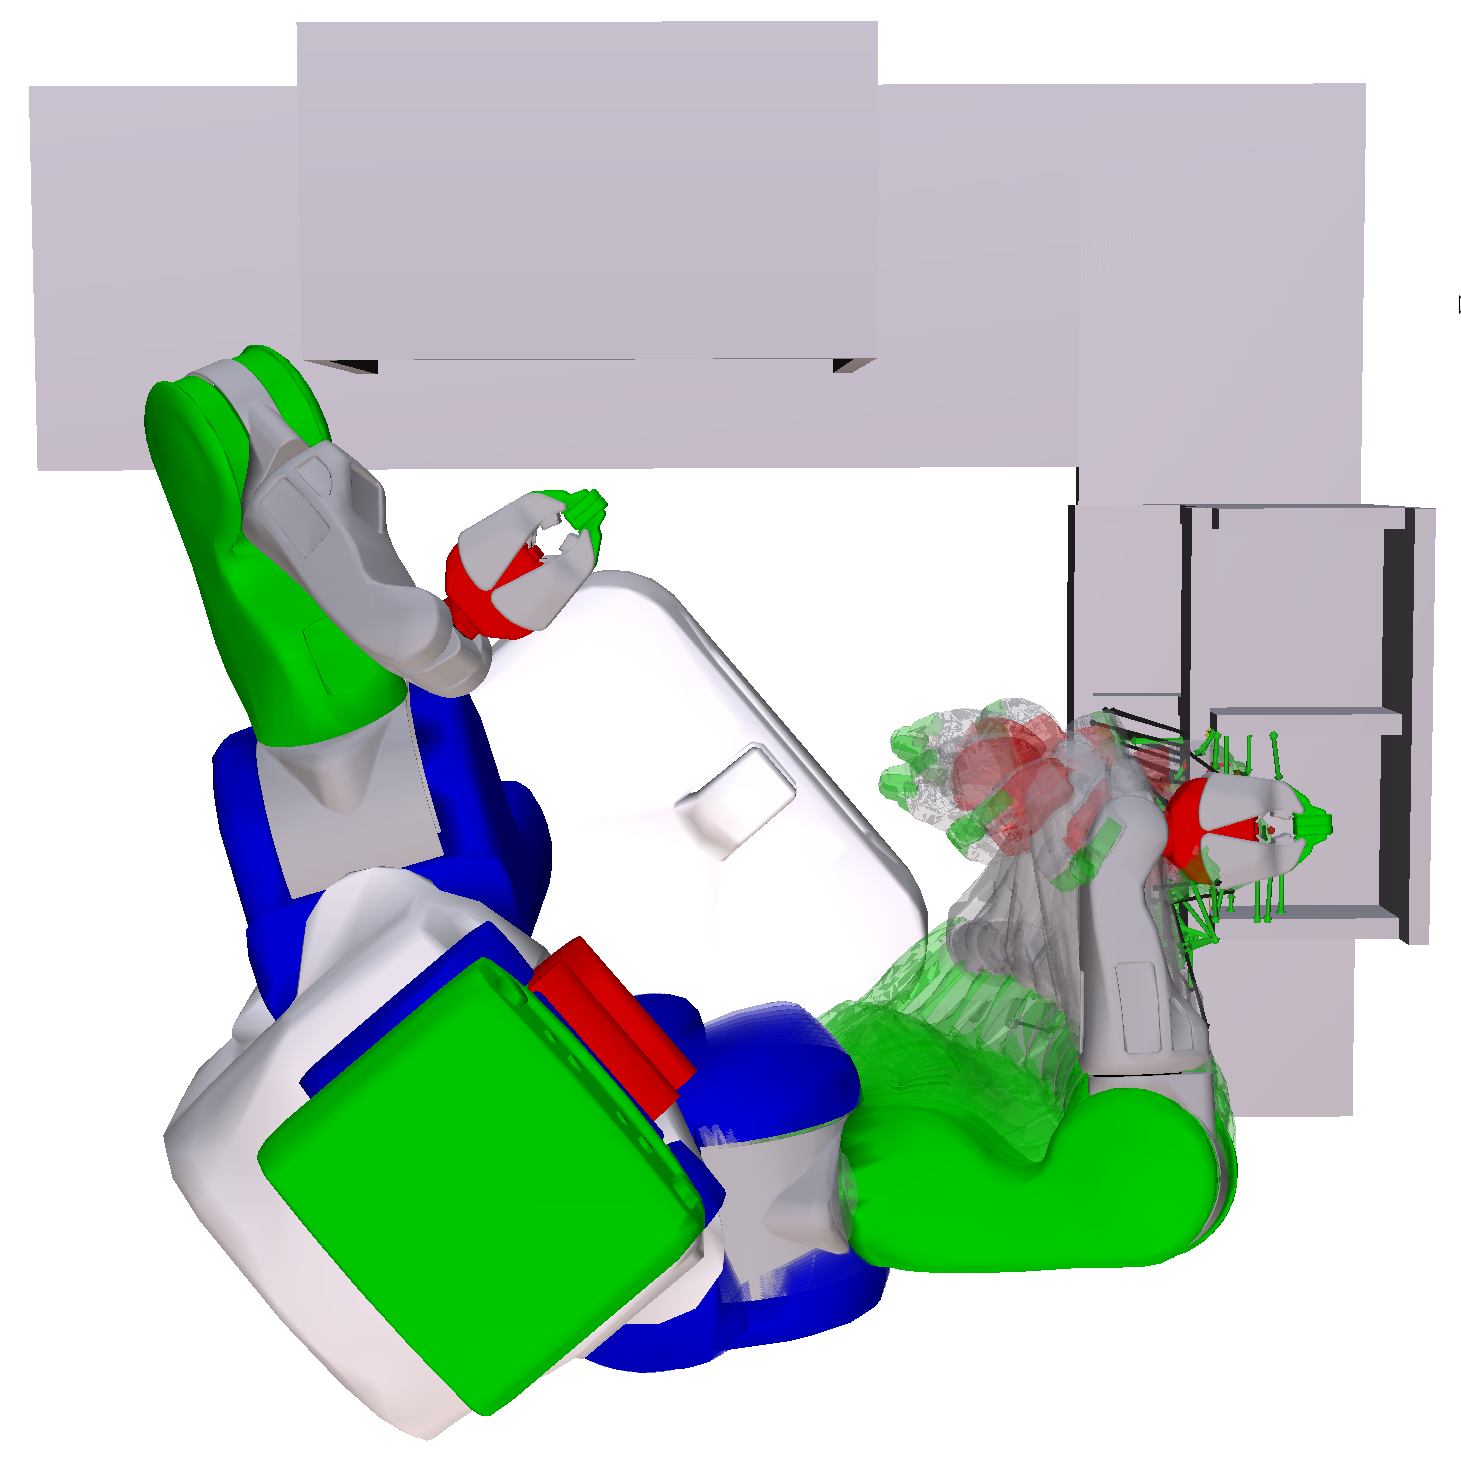
\includegraphics[width=0.18\linewidth]{figure/benchmark/industrial2.png}}
\caption{The PR2 benchmarks for right arm planning with 22 links.}
\label{fig:benchmarks2}
\end{figure*}


\begin{figure*}[t]
\centering
\subfloat[hotel]{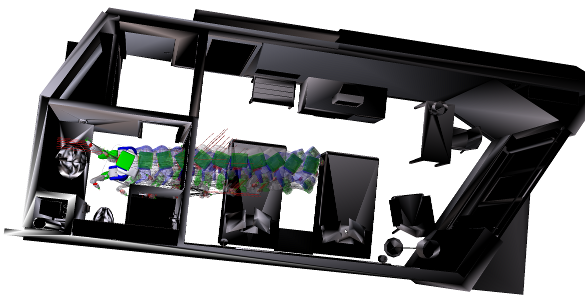
\includegraphics[width=0.35\linewidth]{figure/benchmark/hotel.png}}
\subfloat[kitchen]{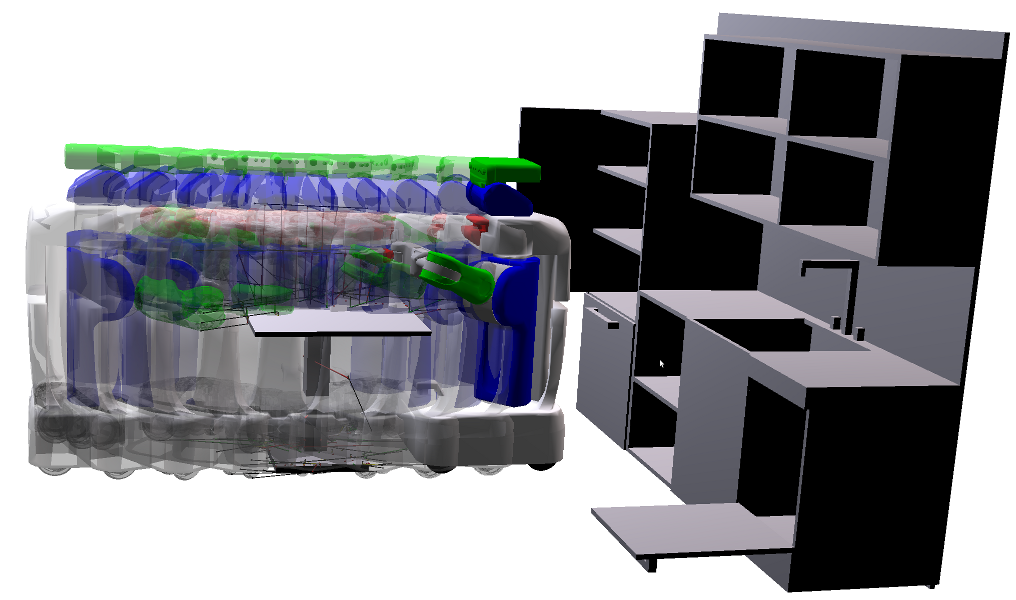
\includegraphics[width=0.33\linewidth]{figure/benchmark/kitchen10.png}} \\
\subfloat[kitchen2]{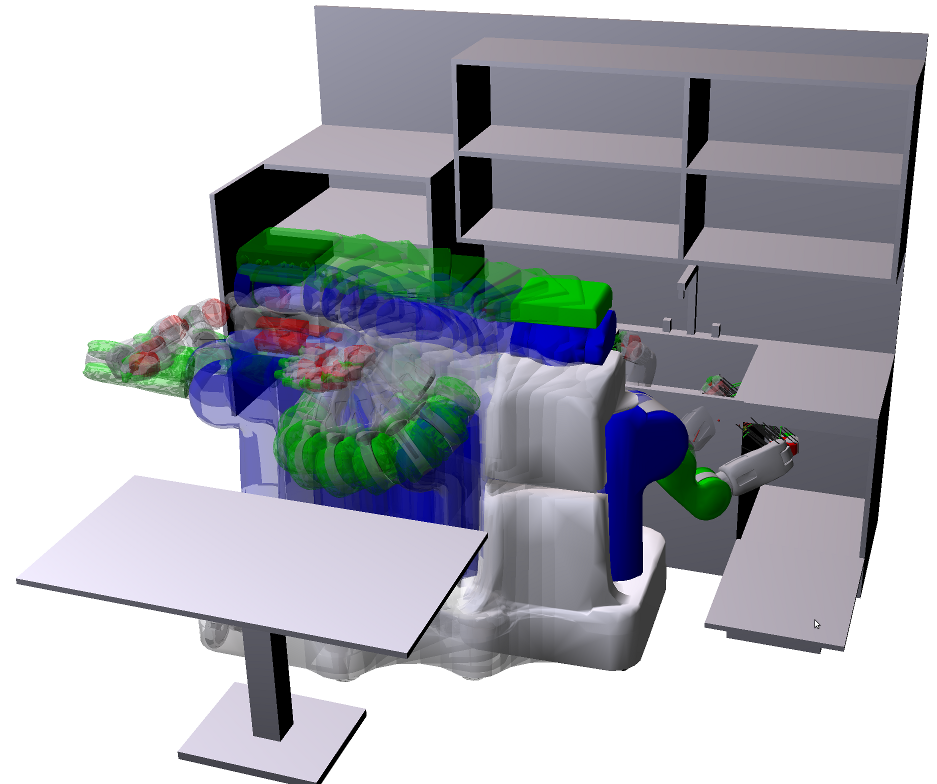
\includegraphics[width=0.24\linewidth]{figure/benchmark/kitchen.png}}
\subfloat[livingroom]{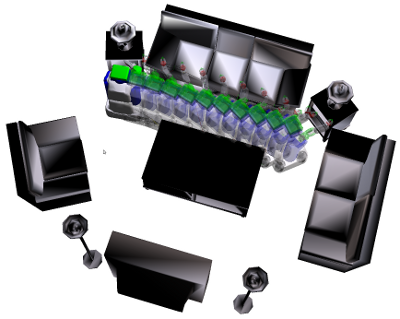
\includegraphics[width=0.24\linewidth]{figure/benchmark/livingroom.png}}
\subfloat[livingroom2]{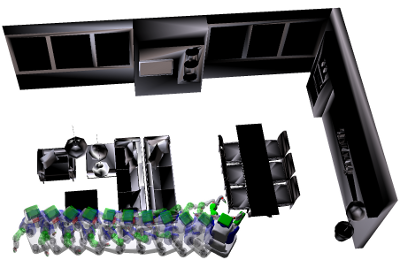
\includegraphics[width=0.30\linewidth]{figure/benchmark/livingroom2.png}}
\caption{The PR2 benchmarks for full-body planning with 88 links.}
\label{fig:benchmarks3}
\end{figure*}




\section{Conclusion}
In this paper, we have introduced novel features for trajectory effectiveness and demonstrated the trajectory effectiveness prediction algorithm based on these features. We showed the the accuracy of the prediction algorithm on different planning tasks in various benchmarks. Additionally, we showed initial results on transferring the learned classifier to other benchmarks.

This work serves as a baseline for initial trajectory selection for trajectory optimization based motion planning. In future work, we would like to consider more combinations of trajectory features and explore more criteria for trajectory evaluation, including running time, objective value and cost for violated constraints. Moreover, we plan to use regression algorithms to predict the optimization algorithm's running time and final outcome when using a given trajectory as initial guess. Finally, we will integrate the prediction algorithm with trajectory optimization in order to improve both the performance and quality of the planning algorithm.


\section*{Acknowledgments}
This research has been funded in part by a Darpa Young Faculty Award, and by a Sloan Fellowship.

\bibliographystyle{IEEEtran}
\bibliography{icra}

\end{document}
